\documentclass[aspectratio=169,11pt]{beamer}

% Shared style (ib-tutorials.sty at the repo root).
\makeatletter\def\input@path{{./}{../}}\makeatother
\usepackage{ib-tutorials}

\usepackage[utf8]{inputenc}
\usepackage{amsmath,amssymb}
\usepackage{booktabs}
\usepackage{array}
\usepackage{graphicx}
\usepackage{xcolor}
\usepackage{listings}
\usepackage{tikz}
\usetikzlibrary{arrows.meta,positioning,shapes.geometric,fit,calc}
\usepackage{hyperref}

\newcommand{\sourcecredit}[1]{\vfill\begin{flushright}\tiny\textcolor{DarkGray}{#1}\end{flushright}}
\newcolumntype{L}[1]{>{\raggedright\arraybackslash}p{#1}}

% Part X: every slide carries the legacy label.
\setbeamertemplate{background}{\begin{tikzpicture}[remember picture,overlay]
  \node[anchor=north east,font=\tiny\sffamily,text=DarkGray,fill=LightGray!50,rounded corners=1pt,inner sep=2pt]
    at ([xshift=-2mm,yshift=-1.2mm]current page.north east) {LEGACY \textbullet\ Part X, archive};
\end{tikzpicture}}

\lstset{
  basicstyle=\ttfamily\scriptsize\color{BlackGray},
  keywordstyle=\color{NavyBlue}\bfseries,
  commentstyle=\color{DarkGray}\itshape,
  stringstyle=\color{OliveGreen},
  showstringspaces=false,
  columns=fullflexible,
  keepspaces=true,
  frame=single,
  framerule=0.4pt,
  rulecolor=\color{LightGray},
  backgroundcolor=\color{LightGray!30},
  xleftmargin=0.25em,
  xrightmargin=0.25em,
  breaklines=true,
  breakatwhitespace=true
}
\lstdefinestyle{shell}{morecomment=[l]{\#}}
\lstdefinestyle{cpp}{language=C++,morekeywords={nullptr}}
\lstdefinestyle{cpptiny}{language=C++,morekeywords={nullptr},basicstyle=\ttfamily\tiny\color{BlackGray}}
\lstdefinestyle{make}{morecomment=[l]{\#}}
\lstdefinestyle{maketiny}{morecomment=[l]{\#},basicstyle=\ttfamily\tiny\color{BlackGray}}
\lstdefinestyle{plaintiny}{basicstyle=\ttfamily\tiny\color{BlackGray}}

\title[X4 Course logistics]{X4. Course logistics, 2013--2024}
\subtitle{The courses, lab series and workshops behind these notes: their schedules, topics, software, accounts, project milestones and grading weights, and where each one's material is now; labelled legacy}
\author[Miller]{Laura A. Miller}
\institute[UArizona]{Department of Mathematics, University of Arizona}
\date{Using IB Software \textbullet\ Part X, archive \textbullet\ Chapter X4}


\begin{document}

% 1
\begin{frame}[plain]
\maketutorialtitlepanel{%
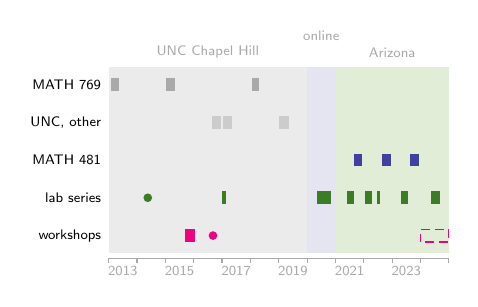
\begin{tikzpicture}[x=0.36cm, y=0.48cm, every node/.style={font=\tiny\sffamily, inner sep=1pt}]
  \fill[LightGray!45] (0,0.45) rectangle (7,-4.45);
  \fill[NavyBlue!10] (7,0.45) rectangle (8,-4.45);
  \fill[OliveGreen!12] (8,0.45) rectangle (12,-4.45);
  \node[text=DarkGray] at (3.5,0.85) {UNC Chapel Hill};
  \node[text=DarkGray] at (7.5,1.3) {online};
  \node[text=DarkGray] at (10,0.85) {Arizona};
  \node[anchor=east] at (-0.15,0) {MATH 769};
  \node[anchor=east] at (-0.15,-1) {UNC, other};
  \node[anchor=east] at (-0.15,-2) {MATH 481};
  \node[anchor=east] at (-0.15,-3) {lab series};
  \node[anchor=east] at (-0.15,-4) {workshops};
  % MATH 769: 2013, 2015, 2018
  \fill[DarkGray] (0.07,-0.17) rectangle (0.35,0.17);
  \fill[DarkGray] (2.02,-0.17) rectangle (2.33,0.17);
  \fill[DarkGray] (5.04,-0.17) rectangle (5.30,0.17);
  % other UNC courses: 768 and 564 (2016), 60H (2017), 762 and 60 (2019)
  \fill[DarkGray!60] (3.64,-1.17) rectangle (3.96,-0.83);
  \fill[DarkGray!60] (4.03,-1.17) rectangle (4.35,-0.83);
  \fill[DarkGray!60] (6.02,-1.17) rectangle (6.35,-0.83);
  % MATH 481: fall 2021, 2022, 2023
  \fill[NavyBlue!75] (8.64,-2.17) rectangle (8.95,-1.83);
  \fill[NavyBlue!75] (9.64,-2.17) rectangle (9.95,-1.83);
  \fill[NavyBlue!75] (10.64,-2.17) rectangle (10.95,-1.83);
  % lab series, tutorials and groups
  \fill[OliveGreen] (1.38,-3) circle (0.55mm);
  \fill[OliveGreen] (4.00,-3.17) rectangle (4.13,-2.83);
  \fill[OliveGreen] (7.36,-3.17) rectangle (7.86,-2.83);
  \fill[OliveGreen] (8.42,-3.17) rectangle (8.65,-2.83);
  \fill[OliveGreen] (9.05,-3.17) rectangle (9.30,-2.83);
  \fill[OliveGreen] (9.48,-3.17) rectangle (9.57,-2.83);
  \fill[OliveGreen] (10.33,-3.17) rectangle (10.56,-2.83);
  \fill[OliveGreen] (11.37,-3.17) rectangle (11.68,-2.83);
  % workshops and talks
  \fill[RubineRed] (2.70,-4.17) rectangle (3.04,-3.83);
  \fill[RubineRed] (3.68,-4) circle (0.55mm);
  \draw[RubineRed,densely dashed] (11.0,-4.17) rectangle (12.0,-3.83);
  % axis
  \draw[DarkGray] (0,-4.6) -- (12,-4.6);
  \foreach \x in {0,...,12} \draw[DarkGray] (\x,-4.6) -- (\x,-4.72);
  \foreach \x/\yr in {0/2013,2/2015,4/2017,6/2019,8/2021,10/2023} \node[text=DarkGray,anchor=north] at (\x+0.5,-4.74) {\yr};
\end{tikzpicture}}
\end{frame}

% 2
\begin{frame}{What this chapter is for}
\label{fr:use}
\begin{columns}[T,onlytextwidth]
\begin{column}{0.575\textwidth}
\footnotesize
\begin{itemize}\setlength{\itemsep}{0.5pt}
  \item \al{Reading old course material.} From 2013 to 2024 IB software was taught in courses at UNC Chapel Hill and the University of Arizona, in lab series and in workshops. Their decks and handouts speak of Sakai, WordPress posts, Dropbox folders, Thursday coding days and project drafts. This chapter keeps the logistics behind them: course structure, schedules, topics, software, kinds of accounts, project milestones and grading weights.
  \item \al{Legacy.} Dates are given as the sources state them; where a source is silent (who attended, how many sessions), the slide says so. Nothing here is needed for the other chapters.
  \item \al{Privacy.} No contact details, rooms, office hours, class keys, course-site numbers, meeting links, rosters, sign-up sheets, grades or students' names. Students' projects appear only as themes, the homework only as logistics.
\end{itemize}
\end{column}
\begin{column}{0.395\textwidth}
\begin{punchbox}
\scriptsize \textbf{Where the material went}
\begin{itemize}\setlength{\itemsep}{1pt}
  \item The homework as assigned: Appendix C, slides 6--9 (``The course homework as it was assigned (1/4)'' to ``(4/4)''). Appendix C adds no answers; the chapters that print some are listed in Appendix C, slide 3.
  \item The course example folders: chapter X3, slides 37--39 (``The map (1/3)'' to ``(3/3)''), and chapter 36.
  \item Clusters and accounts: chapter X1. Installs: chapter X2.
  \item The recordings: chapter 0.1, slides 8--10 (``Lecture videos (1 of 3)'' to ``(3 of 3)'').
\end{itemize}
\end{punchbox}
\vspace{1mm}
\scriptsize Today's way to do what these courses did: chapters 1--3 (Puma, autoibamr, CMake), Part II (IB2d) and Parts III--V (IBAMR, IBFE, VisIt).
\end{column}
\end{columns}
\sourcecredit{The instructor's syllabi, Lecture 1 decks and course folders, 2013--2024; Appendix C; chapters 0.1 and X1--X3.}
\end{frame}

% 3
\begin{frame}{Courses and events, 2013--2024: a timeline}
\label{fr:timeline}
\centering
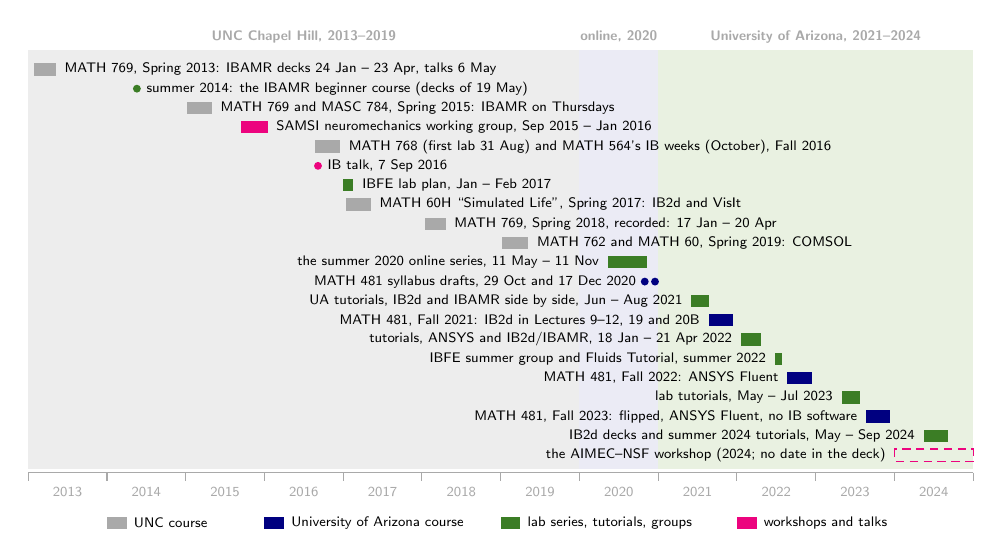
\begin{tikzpicture}[x=1.0cm, y=-0.245cm, every node/.style={font=\tiny\sffamily, inner sep=1pt}]
  \fill[LightGray!40] (0,-1.0) rectangle (7,20.7);
  \fill[NavyBlue!8] (7,-1.0) rectangle (8,20.7);
  \fill[OliveGreen!9] (8,-1.0) rectangle (12,20.7);
  \node[text=DarkGray,font=\tiny\sffamily\bfseries] at (3.5,-1.7) {UNC Chapel Hill, 2013--2019};
  \node[text=DarkGray,font=\tiny\sffamily\bfseries] at (7.5,-1.7) {online, 2020};
  \node[text=DarkGray,font=\tiny\sffamily\bfseries] at (10,-1.7) {University of Arizona, 2021--2024};
  % rows 0-9: labels to the right
  \fill[DarkGray] (0.07,-0.32) rectangle (0.35,0.32); \node[anchor=west] at (0.42,0) {MATH 769, Spring 2013: IBAMR decks 24 Jan -- 23 Apr, talks 6 May};
  \fill[OliveGreen] (1.38,1) circle (0.5mm); \node[anchor=west] at (1.46,1) {summer 2014: the IBAMR beginner course (decks of 19 May)};
  \fill[DarkGray] (2.02,1.68) rectangle (2.33,2.32); \node[anchor=west] at (2.40,2) {MATH 769 and MASC 784, Spring 2015: IBAMR on Thursdays};
  \fill[RubineRed] (2.70,2.68) rectangle (3.04,3.32); \node[anchor=west] at (3.11,3) {SAMSI neuromechanics working group, Sep 2015 -- Jan 2016};
  \fill[DarkGray] (3.64,3.68) rectangle (3.96,4.32); \node[anchor=west] at (4.03,4) {MATH 768 (first lab 31 Aug) and MATH 564's IB weeks (October), Fall 2016};
  \fill[RubineRed] (3.68,5) circle (0.5mm); \node[anchor=west] at (3.76,5) {IB talk, 7 Sep 2016};
  \fill[OliveGreen] (4.00,5.68) rectangle (4.13,6.32); \node[anchor=west] at (4.20,6) {IBFE lab plan, Jan -- Feb 2017};
  \fill[DarkGray] (4.03,6.68) rectangle (4.35,7.32); \node[anchor=west] at (4.42,7) {MATH 60H ``Simulated Life'', Spring 2017: IB2d and VisIt};
  \fill[DarkGray] (5.04,7.68) rectangle (5.30,8.32); \node[anchor=west] at (5.37,8) {MATH 769, Spring 2018, recorded: 17 Jan -- 20 Apr};
  \fill[DarkGray] (6.02,8.68) rectangle (6.35,9.32); \node[anchor=west] at (6.42,9) {MATH 762 and MATH 60, Spring 2019: COMSOL};
  % rows 10-20: labels to the left
  \fill[OliveGreen] (7.36,9.68) rectangle (7.86,10.32); \node[anchor=east] at (7.29,10) {the summer 2020 online series, 11 May -- 11 Nov};
  \fill[NavyBlue] (7.83,11) circle (0.5mm); \fill[NavyBlue] (7.96,11) circle (0.5mm); \node[anchor=east] at (7.76,11) {MATH 481 syllabus drafts, 29 Oct and 17 Dec 2020};
  \fill[OliveGreen] (8.42,11.68) rectangle (8.65,12.32); \node[anchor=east] at (8.35,12) {UA tutorials, IB2d and IBAMR side by side, Jun -- Aug 2021};
  \fill[NavyBlue] (8.64,12.68) rectangle (8.95,13.32); \node[anchor=east] at (8.57,13) {MATH 481, Fall 2021: IB2d in Lectures 9--12, 19 and 20B};
  \fill[OliveGreen] (9.05,13.68) rectangle (9.30,14.32); \node[anchor=east] at (8.98,14) {tutorials, ANSYS and IB2d/IBAMR, 18 Jan -- 21 Apr 2022};
  \fill[OliveGreen] (9.48,14.68) rectangle (9.57,15.32); \node[anchor=east] at (9.41,15) {IBFE summer group and Fluids Tutorial, summer 2022};
  \fill[NavyBlue] (9.64,15.68) rectangle (9.95,16.32); \node[anchor=east] at (9.57,16) {MATH 481, Fall 2022: ANSYS Fluent};
  \fill[OliveGreen] (10.33,16.68) rectangle (10.56,17.32); \node[anchor=east] at (10.26,17) {lab tutorials, May -- Jul 2023};
  \fill[NavyBlue] (10.64,17.68) rectangle (10.95,18.32); \node[anchor=east] at (10.57,18) {MATH 481, Fall 2023: flipped, ANSYS Fluent, no IB software};
  \fill[OliveGreen] (11.37,18.68) rectangle (11.68,19.32); \node[anchor=east] at (11.30,19) {IB2d decks and summer 2024 tutorials, May -- Sep 2024};
  \draw[RubineRed,densely dashed] (11.0,19.68) rectangle (12.0,20.32); \node[anchor=east] at (10.93,20) {the AIMEC--NSF workshop (2024; no date in the deck)};
  % axis
  \draw[DarkGray] (0,20.9) -- (12,20.9);
  \foreach \x in {0,...,12} \draw[DarkGray] (\x,20.9) -- (\x,21.35);
  \foreach \x/\yr in {0/2013,1/2014,2/2015,3/2016,4/2017,5/2018,6/2019,7/2020,8/2021,9/2022,10/2023,11/2024} \node[text=DarkGray] at (\x+0.5,21.9) {\yr};
  % legend
  \fill[DarkGray] (1.0,23.2) rectangle (1.25,23.8); \node[anchor=west] at (1.3,23.5) {UNC course};
  \fill[NavyBlue] (3.0,23.2) rectangle (3.25,23.8); \node[anchor=west] at (3.3,23.5) {University of Arizona course};
  \fill[OliveGreen] (6.0,23.2) rectangle (6.25,23.8); \node[anchor=west] at (6.3,23.5) {lab series, tutorials, groups};
  \fill[RubineRed] (9.0,23.2) rectangle (9.25,23.8); \node[anchor=west] at (9.3,23.5) {workshops and talks};
\end{tikzpicture}
\sourcecredit{Dates as the instructor's syllabi, decks, folders, recordings and the repository's history state them; a bar spans the dated material, not necessarily the whole term.}
\end{frame}

% 4
\begin{frame}{MATH 769, Spring 2013 (1/3): the course}
\label{fr:m769a}
\begin{columns}[T,onlytextwidth]
\begin{column}{0.5\textwidth}
\footnotesize
\begin{itemize}\setlength{\itemsep}{3pt}
  \item \al{Course}: ``MATH 769 Mathematical Modeling II: Biological Fluid Dynamics'', TuTh 12:30--1:45; Spring 2013 (by the folder and the decks' dates).
  \item \al{Level}: no prerequisites stated; ``should be accessible to advanced undergraduate and graduate students from both the mathematical and physical sciences.''
  \item \al{Aim}: ``an introduction to mathematical and numerical methods for current problems in biological fluid dynamics, focusing on the use of the immersed boundary method.''
  \item \al{Texts} (suggested): \emph{Elementary Fluid Dynamics} (1990) and \emph{Mechanics of Swimming and Flying} (1981). ``Supplemental material and codes will be provided throughout the semester. All material will be available on sakai.''
\end{itemize}
\end{column}
\begin{column}{0.47\textwidth}
\footnotesize
\begin{itemize}\setlength{\itemsep}{3pt}
  \item \al{Homework}: ``Students are allowed to work together on the assignments.''
  \item \al{Grading weights}: homework 35\,\%; course project 65\,\% (proposal 10, draft paper and review 10, final paper 25, presentation 20).
  \item \scriptsize\al{Topics} (a selection, in the syllabus's order): introduction (comparative biomechanics, mathematical modeling, dimensional analysis); the equations of fluid motion (Navier--Stokes, ideal fluids, Stokes flow, drag and lift; swimming and flying, seeds and spores); the equations of elasticity (spring--mass--damper, linear elastic models, energy functions, resonance); fluid--structure interaction (vortex shedding, immersed boundary methods, regularized Stokeslets; flapping wings, swimming bacteria, twirling seeds); ``If time permits'': muscle mechanics, neuromechanics.
\end{itemize}
\end{column}
\end{columns}
\sourcecredit{MATH 769 syllabus, Spring 2013 (room and contact lines withheld).}
\end{frame}

% 5
\begin{frame}{MATH 769, Spring 2013 (2/3): the project and the term}
\label{fr:m769p}
\begin{columns}[T,onlytextwidth]
\begin{column}{0.4\textwidth}
\footnotesize
\begin{itemize}\setlength{\itemsep}{3pt}
  \item \al{The project}: in pairs or alone, ``a semester long modeling project''.
  \item ``A list of possible projects will be discussed during the second week of class.''
  \item \al{Its weight}: 65\,\% of the grade (proposal 10, draft paper and review 10, final paper 25, presentation 20).
\end{itemize}
\end{column}
\begin{column}{0.57\textwidth}
\scriptsize
\renewcommand{\arraystretch}{1.08}
\setlength{\tabcolsep}{3pt}
\begin{tabular}{@{}L{0.17\linewidth}L{0.2\linewidth}L{0.57\linewidth}@{}}
\toprule
date & step & format \\
\midrule
31 Jan & proposal & ``please use NSF postdoc proposal format'' \\
9 Apr & draft paper & as ``a paper to be submitted to the Journal of Theoretical Biology'' \\
16 Apr & review & ``the review of the paper will be graded'' \\
25 Apr & final paper & ``on the last day of class'' \\
6 May, 12:00 & presentations & 20 minutes per group, in the final exam period \\
\bottomrule
\end{tabular}
\end{column}
\end{columns}

\vspace{2mm}
\centering
\begin{tikzpicture}[x=0.125cm, y=1cm, every node/.style={font=\tiny\sffamily, inner sep=1pt}]
  \fill[LightGray!40] (21,-0.75) rectangle (32,1.45);
  \fill[LightGray!15] (32,-0.75) rectangle (60,1.45);
  \fill[LightGray!40] (60,-0.75) rectangle (91,1.45);
  \fill[LightGray!15] (91,-0.75) rectangle (121,1.45);
  \fill[LightGray!40] (121,-0.75) rectangle (130,1.45);
  \foreach \x/\m in {26.5/January,46/February,75.5/March,106/April,125.5/May} \node[text=DarkGray] at (\x,1.6) {\m};
  \draw[DarkGray] (21,0) -- (130,0);
  \foreach \d/\t in {24/new-force install, 29/input files; VisIt, 36/parameters; BCs, 43/springs; targets, 50/bending, 57/forces; jellyfish, 78/3D, 94/IBAMR's examples, 101/IBFE, 113/output to MATLAB}
    {\fill[DarkGray] (\d,0) circle (0.45mm); \node[anchor=south west, rotate=48, text=BlackGray] at (\d,0.07) {\t};}
  \foreach \d/\t in {31/proposal, 99/draft, 106/review, 115/final paper, 126/talks}
    {\node[diamond, fill=NavyBlue, inner sep=0.8pt] at (\d,0) {}; \node[text=NavyBlue, anchor=north] at (\d,-0.15) {\t};}
  \node[diamond, fill=OliveGreen, inner sep=0.8pt] at (50,0) {}; \node[text=OliveGreen, anchor=north] at (50,-0.15) {homework 1 due};
  \node[text=DarkGray] at (75,-0.6) {dots: the IBAMR decks (slide \ref{fr:m769b}); diamonds: the project's steps and the first homework};
\end{tikzpicture}
\sourcecredit{MATH 769 syllabus, Spring 2013; the dates of the course's decks and of its first homework.}
\end{frame}

% 6
\begin{frame}{MATH 769, Spring 2013 (3/3): the IBAMR lectures, date by date}
\label{fr:m769b}
\tiny
\renewcommand{\arraystretch}{1.1}
\setlength{\tabcolsep}{3pt}
\begin{tabular}{@{}L{0.17\textwidth}L{0.42\textwidth}L{0.24\textwidth}L{0.11\textwidth}@{}}
\toprule
date (2013) & deck: title as printed, or file name & topic & now (chapter) \\
\midrule
24 Jan (file) & \code{IBAMR\_Forces\_Install.ppt} (in \code{examples}) & installing the ``new force'' IBAMR & X2, X1 \\
29 Jan (slide: ``January 29, 2012'') & ``Immersed boundary tutorial continued''; \code{IBAMR\_InputVisualization-1.ppt} & what the input files do; first VisIt & 6, 26; X3 \\
5 Feb & ``IBAMR -- parameter changes''; ``IBAMR boundary conditions'' & parameters; boundary conditions & 8a, 7 \\
12 Feb & ``Changing spring lengths, stiffnesses and target points''; ``IBAMR with multiple boundaries'' & springs, targets, several structures & 9a \\
19 Feb & ``Bending in IBAMR'' & beams, curvature & 10 \\
26 Feb (slide: ``February 26, 2012'') & ``IBAMR Forces''; ``Specific example of jellyfish swimming by prescribing curvature'' & forces; a 2D jellyfish & 11, 10 \\
19 Mar (file) & \code{Math769\_3D.ppt} & 3D & 12 \\
4 Apr & ``IBAMR Examples'' & a tour of IBAMR's own examples & 15 \\
11 Apr & ``IBAMR with FE'' & the first IBFE lecture & 17, 28 \\
23 Apr & ``Converting IBAMR output to Matlab and analyzing it'' & output to MATLAB & 11, 33 \\
9 Oct (file; no date on the slides) & ``Creating your own spring function in IBAMR'' & your own spring law & 9b \\
\bottomrule
\end{tabular}

\vspace{2mm}
\scriptsize
\begin{itemize}\setlength{\itemsep}{2pt}
  \item \al{Beside the decks}, example folders and zips (dated 19--26 February 2013 where dated): moving bristles, multiple boundaries, changing spring lengths, 2D beams and a jellyfish with curvature, a fruit fly at Re 10, \code{ex0}, \code{3D}; and Linux install notes (30 April). Today the bristles are IB/04 and the multiple boundaries IB/07 (Appendix C, slide 7); the curvature examples are IB/09 and IB/10 (chapter X3, slide 37, ``The map (1/3)''); changing spring lengths is the topic of IB/06 (growing springs).
  \item \al{Dates}: three title slides say 2012 (one of 29 January, two of 26 February); their files and the course are 2013. The springs deck also exists as a \code{MATH768\_} file, which says MATH 769 on its slide.
\end{itemize}
\sourcecredit{Title slides and file dates of the MATH 769 decks, Spring 2013, and the course folder's listing; Appendix C, slide 7; chapter X3, slide 37.}
\end{frame}

% 7
\begin{frame}{The 2013 homework, and where its problems are now}
\label{fr:hw2013}
\begin{columns}[T,onlytextwidth]
\begin{column}{0.53\textwidth}
\footnotesize
\renewcommand{\arraystretch}{1.25}
\setlength{\tabcolsep}{3pt}
\begin{tabular}{@{}L{0.24\linewidth}L{0.72\linewidth}@{}}
\toprule
header & ``Homework \#1, MATH 564''; ``Due: Tuesday, February 19, 2013'' \\
where filed & the MATH 769 folder of Spring 2013; the sources do not say why it is headed MATH 564 \\
content & five IBAMR problems on two course examples, then pencil-and-paper fluids problems \\
where run & on ``the new force installation of IBAMR'', on a lab server (name withheld), or on ``killdevil (kure)'' \\
handed in & screenshots of the plots, named by problem (``as HW1 problem 1''); problem 2 is a calculation \\
course site & Sakai: ``All material will be available on sakai'' (the 2013 syllabus) \\
\bottomrule
\end{tabular}
\end{column}
\begin{column}{0.44\textwidth}
\begin{homebox}
\footnotesize \textbf{The problems are in Appendix C}, slide 7 (``The course homework as it was assigned (2/4): the IBAMR course, 2013''), with today's examples (IB/04, IB/07) and chapters (8b, 9a, 26). The pencil-and-paper problems belong to the theory series, \emph{Fluid Dynamics and IBM Theory}. The answer key is not reproduced anywhere.
\end{homebox}
\vspace{2mm}
\footnotesize How the homework ran on the lab server and the cluster: chapter X1, slide ``A 2013 homework on the lab server''.
\end{column}
\end{columns}
\sourcecredit{Homework 1 of Spring 2013 (its problem statements only; the answer key not used); MATH 769 syllabus, Spring 2013; Appendix C, slide 7; chapter X1.}
\end{frame}

% 8
\begin{frame}{Summer 2014: the IBAMR beginner course}
\label{fr:summer2014}
\begin{columns}[T,onlytextwidth]
\begin{column}{0.52\textwidth}
\footnotesize
\begin{itemize}\setlength{\itemsep}{3pt}
  \item \al{The decks}: ``0-IBAMR Tutorial UNC Edition'' (title slide ``May 19, 2014''): the IB method and its numerics; ``0A - IBAMR Tutorial: UNC Edition'' (``May 19, 2014''): getting started on Kure, by which time each participant was to have a Kure account; a later, undated copy, ``1-IBAMR Tutorial UNC Edition''. Their author is not stated.
  \item \al{The notes} (ibamr-101, built 26 May 2014) say that they come from an IBAMR beginner course which the instructor first organized at UNC in the summer of 2014; their author, Dennis Evangelista, is credited in chapter 0.1, slide 5 (``Contributors'').
  \item \al{Prerequisites} (the notes): ssh, sftp, VisIt, a Kure account through Onyen services, and the VPN from home.
\end{itemize}
\end{column}
\begin{column}{0.45\textwidth}
\scriptsize
\begin{itemize}\setlength{\itemsep}{2pt}
  \item \al{The first run}: the FlowTank example (a 2D triangle in a 10 cm channel; a 3D cone) from the public tutorials folder, submitted with \code{bsub} on Kure, as a test of access; what the example does was left for the next session.
  \item \al{Not stated}: the course's dates, its audience and its number of sessions; the notes end with an empty section for the second Tuesday's session.
\end{itemize}
\begin{punchbox}
\scriptsize \textbf{A wrong line in the 2014 notes}: they call IBAMR primarily a two-dimensional tool. IBAMR runs in 2D and in 3D, as the notes' own 3D cone shows.
\end{punchbox}
\al{Also from 2014}, and used by the lab: Nick Battista's Kure and KillDevil instructions (August) and his gmsh tutorial (24 September); Alex Hoover's IBFE tutorials (2013--15).

\vspace{1mm}
\al{Now}: the first run, chapters 1--3; the overview of the method, chapter 5; the 2014 handouts and the FlowTank run, chapter X1 (slides ``The first-simulation handouts (1/2): UNC, 2014--2018'' and ``The FlowTank first run (2014)'').
\end{column}
\end{columns}
\sourcecredit{The ``IBAMR Tutorial: UNC Edition'' decks (19 May 2014); the ibamr-101 notes (built 26 May 2014); chapters 0.1 and X1.}
\end{frame}

% 9
\begin{frame}{MATH 769 and MASC 784, 2015 (1/4): the course}
\label{fr:m769c}
\begin{columns}[T,onlytextwidth]
\begin{column}{0.5\textwidth}
\footnotesize
\begin{itemize}\setlength{\itemsep}{3pt}
  \item \al{Course}: Spring 2015, with the 2013 title, aim, level and texts (the description now also names muscle models); TuTh 12:30--1:45. Lecture 1 (8 January 2015) is headed ``MATH 769 and MASC 784 / Mathematical modeling II: Biofluids'', a cross-listing with marine sciences.
  \item \al{Two kinds of class}: Tuesdays, ``lectures on topics in biofluids''; Thursdays, ``in-class programming activities'' with IBAMR: ``Please come with your laptop on Thursdays and be ready to code.''
  \item \al{Homework on WordPress}: one post a week on the course's WordPress site, due at 11:59 pm on Tuesdays and titled ``Homework 1, Homework 2, etc.''; ``You must comment on two of your classmate's posts each week'' (comments due on Friday).
\end{itemize}
\end{column}
\begin{column}{0.47\textwidth}
\footnotesize
\begin{itemize}\setlength{\itemsep}{3pt}
  \item \al{Grading weights}: homework 35\,\%; project 65\,\% (proposal 10, peer review 10, final paper 25, presentation 20).
  \item \al{Accounts}: Sakai (course documents), WordPress (homework), WebAssign (with a class key, withheld), Kure.
  \item \al{Topics} (a selection, in order): introduction; the equations of fluid motion; fluid forces I (estimates of lift and drag, quasi-steady) and II (inviscid and viscous theory); the equations of elasticity; muscle mechanics; neuromechanics.
\end{itemize}
\end{column}
\end{columns}
\sourcecredit{MATH 769 syllabus, Spring 2015; MATH 769 Lecture 1 (8 January 2015), slides 1--9 (contact lines, class key and course site withheld).}
\end{frame}

% 10
\begin{frame}{MATH 769 and MASC 784, 2015 (2/4): the project}
\label{fr:m769c2}
\begin{columns}[T,onlytextwidth]
\begin{column}{0.44\textwidth}
\footnotesize
\al{The project}: pairs allowed, but ``If working in pairs, then each person should outline an independent subproject that is to be proposed as their own wordpress entry.''
\end{column}
\begin{column}{0.53\textwidth}
\scriptsize
\renewcommand{\arraystretch}{1.12}
\setlength{\tabcolsep}{3pt}
\begin{tabular}{@{}L{0.24\linewidth}L{0.7\linewidth}@{}}
\toprule
date & step \\
\midrule
3 Feb & proposals, as WordPress entries \\
7 Apr & the draft: Journal of Theoretical Biology format, a PDF on the site \\
14 Apr & reviews, as comments on the site \\
23 Apr & the final paper \\
1 May, 12:00--3:00 p.m. & 20-minute group talks \\
\bottomrule
\end{tabular}
\end{column}
\end{columns}
\sourcecredit{MATH 769 syllabus, Spring 2015; MATH 769 Lecture 1 (8 January 2015), slides 3, 8, 11 and 12--37 (the class key and the course site withheld).}
\end{frame}

% 10b
\begin{frame}{MATH 769 and MASC 784, 2015 (3/4): week 1}
\label{fr:m769c3}
\begin{columns}[T,onlytextwidth]
\begin{column}{0.5\textwidth}
\footnotesize
\al{The First Week Checklist} (Lecture 1, slide 11): ``Please take a screenshot of your computer with a terminal opened that is logged into kure.'' A second screenshot of VisIt, both posted on the WordPress site as ``Week 1''; find the course on Sakai; install FileZilla or another sftp program ``to move files on and off kure.''

\vspace{2mm}
\begin{punchbox}
\scriptsize \textbf{A slip and a caveat in Lecture 1}: the WebAssign row is labelled ``BIOL 226, section 001'', copied from another course; and slide 28 says of the CFL condition ``In IBAMR, we rarely have to worry about this.'', which chapter 5 (slide 43, ``The CFL condition in our runs'') finds true for this series' runs, until a fast flow on a fine grid makes the limit bind.
\end{punchbox}
\end{column}
\begin{column}{0.47\textwidth}
\footnotesize
\al{The rest of Lecture 1} (slides 12--37): the IB method and its numerics, with two MATLAB demos, \code{stiff\_ode\_example} and \code{heat\_equation} (``Download stiff\_ode\_example.m from google docs''). \al{Now}: the method, chapter 5; the demos, chapter 4d and Appendix A.
\end{column}
\end{columns}
\sourcecredit{MATH 769 syllabus, Spring 2015; MATH 769 Lecture 1 (8 January 2015), slides 3, 8, 11 and 12--37 (the class key and the course site withheld).}
\end{frame}

% 11
\begin{frame}{MATH 769 and MASC 784, 2015 (4/4): lecture by lecture}
\label{fr:m769d}
\tiny
\renewcommand{\arraystretch}{1.12}
\setlength{\tabcolsep}{3pt}
\begin{tabular}{@{}L{0.36\textwidth}L{0.1\textwidth}L{0.3\textwidth}L{0.17\textwidth}@{}}
\toprule
lecture (title as filed; title slide if it differs) & date (2015) & example or data handed out & now \\
\midrule
1 -- Introduction & 8 Jan & MATLAB demos \code{stiff\_ode\_example}, \code{heat\_equation} & chapters 5, 4d; App.~A \\
2 (a 1964 reading, a PDF) & 11 Jan & -- & not used \\
3 -- Getting started with IBAMR (``January 15, 2015'') & 15 Jan & \code{FlowTank.zip} & chapters 1--3; X1 \\
4 -- WritingPaper; 4A -- Graph supplement & 20 Jan & -- & writing; graphs \\
5 IBAMR Input Files (``IBAMR Tutorial -- Getting Started'') & 22 Jan & -- & chapter 6 \\
7: Boundary Conditions and Changing Parameters & 29 Jan -- 5 Feb & -- & chapters 7, 8a \\
8: Changing Target Point Positions and Springs & 1--3 Feb & \code{Example\_2DMovingCylinders.zip}, \code{Example\_2DSprings.zip} (``Go to sakai and download \ldots'') & chapter 9a; IB/04, IB/06 \\
9: Changing Parameters (``Lecture 7 -- Dimensionless numbers and how to start changing things'') & 5 Feb & -- & chapter 8b \\
10 VISIT -- How to make it look better & 10 Feb & \code{2plate\_viz\_IB2d.zip}: ``data for a 2D simulation of two flapping plates'' & chapter 26 \\
11 -- Visit 3D & 24 Feb & -- & chapter 27 \\
12: Changing Target Positions, Springs, and Multiple Boundaries & 3 Mar & \code{Example\_2Dmoving\_plates.zip} & chapter 9a; IB/07 \\
15 -- Outputting forces (``Output and Analyze Forces'') & 19 Mar & -- & chapter 11 \\
\bottomrule
\end{tabular}

\vspace{2mm}
\footnotesize Lectures 6, 13 and 14 have no file in the folder. The dates are the files' creation dates (title-slide dates for Lectures 1 and 3), not class dates; the syllabus put the IBAMR programming on Thursdays. Lecture 12's exercise on stretching and shrinking plates is in Appendix C, slide 8 (``The course homework as it was assigned (3/4): the IBAMR courses, 2015--2020''), and in chapter 9a.
\sourcecredit{The MATH 769 Spring 2015 lecture folder (creation dates) and the decks' title slides; Appendix C, slide 8; dates are the files' creation dates (UTC).}
\end{frame}

% 12
\begin{frame}{MATH 768, Fall 2016, and IB weeks in MATH 564 (1/3): MATH 768, the course}
\label{fr:m768}
\footnotesize
\begin{itemize}\setlength{\itemsep}{3pt}
  \item \al{Course}: the syllabus (24 August 2016) is headed ``MATH 768 Mathematical Modeling II: Biological Fluid Dynamics'', the MATH 769 title; MWF 10:10--11:00 am. Description, level and texts as MATH 769 (the texts now ``Supplementary'').
  \item \al{The project}: ``A list of possible projects will be discussed during the third week of class.'' 14 Sep, proposals; 9 Nov, the draft (Journal of Theoretical Biology format); 16 Nov, reviews; 5 and 7 Dec, the talks (``Each group will give a 15 minute presentation during the final exam period''); 16 Dec, 8--11 am, the final exam slot: the paper, by e-mail.
  \item \al{Topics} (a selection, in order): fluid mechanics (diffusion, advection, Navier--Stokes); structures in a flow (lift and drag; the elasticity of organisms); the biology of movement (muscle mechanics, neuromechanics, muscle activation, plant movement); the mathematics of FSI (Stokes, inviscid, full Navier--Stokes); the analysis of movement (ecomechanics, efficiency, validation by PIV).
  \item \al{Grading weights}: homework 35\,\%; project 65\,\% (proposal 10, peer review 10, final paper 25, presentation 20).
\end{itemize}
\sourcecredit{MATH 768 syllabus, Fall 2016 (contact lines withheld).}
\end{frame}

% 12b
\begin{frame}{MATH 768, Fall 2016, and IB weeks in MATH 564 (2/3): MATH 768, the first lab}
\label{fr:m768lab}
\begin{columns}[T,onlytextwidth]
\begin{column}{0.53\textwidth}
\footnotesize
\al{The first lab}: ``Getting Running on IB2D and IBAMR'' (31 August 2016; the folder's only deck; author not stated):
\begin{enumerate}\setlength{\itemsep}{1pt}
  \item IB2d: clone it with git (\code{module add git/1.8.5.3}; it runs on Kure and KillDevil too); MATLAB as a module, or as a batch job with \code{bmatlab}; IB2d's output folders.
  \item IBAMR: load the module \code{ibamr/3803}, move the files into your \code{netscr} directory, and see the Sakai tutorial for the details.
  \item VisIt: unload \code{ibamr/3803} first (\code{module rm ibamr/3803}), because the two modules conflict.
\end{enumerate}
\end{column}
\begin{column}{0.44\textwidth}
\footnotesize
For readers of the first lab's deck: slide 7 names IB2d's force folder \code{hier\_IB2d\_data}, slide 9 IBAMR's \code{hier\_data\_IB2d}; two programs, two names, both right (chapter X1).

\vspace{2mm}
\begin{punchbox}
\scriptsize \textbf{Now}: IB2d in MATLAB and Python, Part II; IB2d on Kure and \code{bmatlab}, chapter X1 (slides ``IB2d on Kure and KillDevil (2016)'' and ``MATLAB jobs under LSF: bmatlab'').
\end{punchbox}
\end{column}
\end{columns}
\sourcecredit{MATH 768 syllabus, Fall 2016 (contact lines withheld); ``Getting Running on IB2D and IBAMR'' (31 August 2016); chapter X1.}
\end{frame}

% 13
\begin{frame}{MATH 768, Fall 2016, and IB weeks in MATH 564 (3/3): MATH 564}
\label{fr:m564}
\begin{columns}[T,onlytextwidth]
\begin{column}{0.48\textwidth}
\scriptsize
\begin{itemize}\setlength{\itemsep}{2pt}
  \item \al{Course}: ``MATH 564 Mathematical Modeling'', Fall 2016, taught by another instructor (the syllabus of 23 August 2016 is in that instructor's account). The IB weeks come from the instructor's own planning note, ``Course Schedule'' (7 July 2016).
  \item \al{Prerequisites}: the equivalent of MATH 231, 232, 233 and 383 and of COMP 110 or 116, with some familiarity with linear algebra.
  \item \al{Grading weights}: homework 30\,\%; midterm 1, 20\,\%; midterm 2 (the final), 20\,\%; project 30\,\% (drafts 5, final paper 15, presentation 10), in teams of 4--5.
  \item \al{Homework}: on WebAssign, with a key bought from the UNC bookstore.
  \item \al{In the syllabus}: Navier--Stokes, non-dimensionalization and the immersed boundary method in weeks 6--8, among the partial differential equation models.
\end{itemize}
\end{column}
\begin{column}{0.49\textwidth}
\scriptsize
The planning note (``Classes start Tues. Aug. 23''):

\vspace{1mm}
\renewcommand{\arraystretch}{1.05}
\setlength{\tabcolsep}{3pt}
\begin{tabular}{@{}L{0.2\linewidth}L{0.14\linewidth}L{0.59\linewidth}@{}}
\toprule
week of & classes & topic and code, as written \\
\midrule
Sept 26 & 3 & ``Heat equation (LM code)'' \\
Oct 3 & 3 & ``Navier Stokes (PDE) + IBM (Nick code)'' \\
Oct 10 & 3 & ``IBM + Review'' \\
Oct 24 & -- & ``PIV (cross correlation) - (MATPIV code)'' \\
projects & -- & ``Select from 8 projects'' \\
\bottomrule
\end{tabular}

\begin{itemize}\setlength{\itemsep}{1.5pt}
  \item ``Nick code'' is presumably Nick Battista's IB code, IB2d or its MATLAB predecessor; the note does not say which.
  \item The course folder's ``Lectures + Code + Exercises/Heat Equation'' holds a copy of the 2014 ``UNC Edition'' deck.
  \item \al{Now}: the heat equation and the stability lab, chapter 4d; the IB method, chapter 5.
  \item The 2013 homework is also headed MATH 564 (slide \ref{fr:hw2013}).
\end{itemize}
\end{column}
\end{columns}
\sourcecredit{MATH 564 syllabus, Fall 2016 (names, offices and e-mail addresses withheld); the instructor's planning note ``Course Schedule'' (7 July 2016); the course folder's listing.}
\end{frame}

% 14
\begin{frame}{MATH 60H, Spring 2017 (1/3): a first-year seminar}
\label{fr:m60a}
\begin{columns}[T,onlytextwidth]
\begin{column}{0.5\textwidth}
\footnotesize
\begin{itemize}\setlength{\itemsep}{3pt}
  \item \al{Course}: ``MATH 60H Simulated Life'', TuTh 2--3:15, a first-year honors seminar whose theme changed by semester; Lecture 1 (12 January 2017): ``Computational modeling of organisms in a physical environment''.
  \item \al{Theme}: ``The focus of this semester's Simulated Life seminar will be on organisms living within moving fluids.'' Organisms drawn in 3D CAD go into simulations, and ``We will also 3D print these objects and place them inside flow tanks for comparison to simulation.''
  \item \al{First Week Checklist} (Lecture 1, slide 10): a WebAssign account; MATH 60H on Sakai; ``Install MATLAB and take a screenshot of it opened on you[r] computer. Upload that as HW1 on webassign.''
\end{itemize}
\end{column}
\begin{column}{0.47\textwidth}
\footnotesize
\begin{itemize}\setlength{\itemsep}{3pt}
  \item \al{Prerequisites}: ``As with all of the first year seminars at UNC, there are no prerequisites for this course.''
  \item \al{Goals}: 3D models of organs and organisms; ``Run numerical simulations on a remote cluster.''; why the flow around an organism matters for feeding, nutrient exchange, dispersal and survival; flows visualized in experiments and in simulation data. \al{Not goals}: numerical analysis, the mathematics of CAD, ``Teach students how to code.''
  \item \al{Text and software}: \emph{Life's Devices} (1988); MATLAB (Mathematica or Maple allowed), with UNC's download instructions; WebAssign (an account with the Onyen; the class key withheld); Sakai.
\end{itemize}
\end{column}
\end{columns}
\sourcecredit{MATH 60H syllabus, Spring 2017; MATH 60H Lecture 1 (12 January 2017), slides 1--10 (contact lines and class key withheld).}
\end{frame}

% 15
\begin{frame}{MATH 60H, Spring 2017 (2/3): the project and the lectures}
\label{fr:m60b}
\begin{columns}[T,onlytextwidth]
\begin{column}{0.56\textwidth}
\footnotesize
\begin{itemize}\setlength{\itemsep}{3pt}
  \item \al{Grading weights}: homework 30\,\%; participation (in-class assignments) 20\,\%; project 50\,\% (proposal 5, draft 5, review 5, final paper 20, presentation 15).
  \item \al{The project}: alone or in pairs; a 10-page report and a 10-minute talk. 2 Feb, the proposal; 6 Apr, the draft (12 pt, double spaced, page counts per section, ``3-5 references''); 13 Apr, the review; 27 Apr, the final paper; 8 May, the talks (``Monday, May 8th between 12 and 3 p.m.'').
\end{itemize}
\begin{punchbox}
\scriptsize \textbf{Why IB software} (Lecture 1, slides 37, 43, 44): ``Serial code: Four pulses takes about 6 days to run on a desktop.'' ``Parallel and Adaptive Code: 16 pulses takes 1-2 days to run on 16 processors.'' And for 3D IBFE: ``\textasciitilde 6 months for student to learn IBAMR, 6 months to learn IBFE, 6-12 months to choose appropriate parameter values, etc.''
\end{punchbox}
\end{column}
\begin{column}{0.41\textwidth}
\scriptsize
\renewcommand{\arraystretch}{1.05}
\setlength{\tabcolsep}{3pt}
\begin{tabular}{@{}L{0.25\linewidth}L{0.69\linewidth}@{}}
\toprule
date & the lectures folder, as filed \\
\midrule
12 Jan & Lecture 1 \\
24 Jan & ``Project Ideas'' \\
31 Jan & ``DimensionlessParameters\_\allowbreak ProjectIdeas'' \\
2 Feb & ``Lecture 6 - Flow visualization with Visit'' \\
7 Mar & ``Project planning''; ``Van der Pol Oscillators''; ``EulersMethod+Oscillators'' \\
20 Mar & ``How to Write a Research Paper'' \\
29--30 Mar & ``Oscillator Models'' \\
11 Apr & ``Methods and Results'' \\
13--17 Apr & ``Tips on Data Analysis'' \\
20 Apr & ``Scaling and Reynolds Number'' \\
\bottomrule
\end{tabular}

\vspace{1.5mm}
Handouts: \code{VisIt\_basic} (the IB2d rewrite of Lindsay Waldrop's guide) and a PIV homework.
\end{column}
\end{columns}
\sourcecredit{MATH 60H syllabus, Spring 2017; MATH 60H Lecture 1 (12 January 2017), slides 8--9, 37 and 43--44; the MATH 60 Spring 2017 lectures folder (dates); dates are the files' creation dates (UTC).}
\end{frame}

% 16
\begin{frame}{MATH 60H, Spring 2017 (3/3): project ideas, IB2d, VisIt}
\label{fr:m60c}
\begin{columns}[T,onlytextwidth]
\begin{column}{0.495\textwidth}
\footnotesize
\begin{itemize}\setlength{\itemsep}{0.5pt}
  \item \al{``Project Ideas''} (24 Jan): ``Basic idea: Study the flow around or within an organ or organism''; ``First Decision: Do you prefer an experimental or a computational study?'' Both start from 3D scans, then 3D prints (experiment) or meshes (computation). Computation: ``Two dimensional simulation of flow around organ or organism'' in IB2d (``Opportunities to learn version control, contribute to project, etc.''), or a 3D one in IBAMR.
  \item \al{``Lecture 6''} (2 Feb): download VisIt; then, from the Dropbox link of week 4 on Sakai (``Tutorials for Visit''), the sample data (\code{sample\_viz\_IB3d}, \code{viz\_ib2d}); ``Open the tutorial: Visit - How to make it look better''.
\end{itemize}
\begin{homebox}
\scriptsize \textbf{Now}: IB2d, Part II; VisIt and its ``make it look better'' tutorial, chapter 26. PIV is outside this series.
\end{homebox}
\end{column}
\begin{column}{0.475\textwidth}
\scriptsize
\begin{itemize}\setlength{\itemsep}{3pt}
  \item \al{``Project planning''} (7 Mar): the groups and their projects (names withheld). Themes: IB2d with an oscillator model driving the motion; moving boundaries and changing material properties in IB2d (``Step 1: Learn about modifying boundaries in ib2d''); 3D-printed models in a flow tank, with dye or PIV (``Get your models to the Makerspace ASAP!'').
  \item \al{The PIV weeks}: ``Last week of March / beginning of April: PIV of small things (\textasciitilde 3 cm wide) in the small flow tank'', then big things (about 6 inches wide) in the big tank, early to mid April. The deck also gives the steps of a lab-safety registration (not reproduced).
  \item \al{In 2019} the seminar (MATH 60, Spring 2019) kept its theme and goals but simulated with COMSOL Multiphysics on Longleaf (``February 12 -- Logging into remote clusters, using Longleaf''), with weekly entries in an electronic lab notebook: no IB software.
\end{itemize}
\end{column}
\end{columns}
\sourcecredit{``Project Ideas'' (24 January 2017); ``Lecture 6'' (2 February 2017); ``Project planning'' (7 March 2017; names withheld); MATH 60 syllabus, 2019.}
\end{frame}

% 17
\begin{frame}{The IBFE lab plan, Spring 2017}
\label{fr:ibfeplan}
\begin{columns}[T,onlytextwidth]
\begin{column}{0.56\textwidth}
\footnotesize The ``Spring 2017 To Do List'' (public IBFE folder; dated entries from January to 17 February 2017, newest first) ran a weekly plan for the lab, with tasks for lab members (names withheld).

\vspace{1mm}
\scriptsize
\renewcommand{\arraystretch}{1.15}
\setlength{\tabcolsep}{3pt}
\begin{tabular}{@{}L{0.17\linewidth}L{0.79\linewidth}@{}}
\toprule
entry & the plan \\
\midrule
January 2017 & the move from the module \code{ibamr/3803} to \code{ibamr/2016-11}: the examples renamed with the module's suffix (chapters X1, X3) \\
10 Feb & ``Homework for next week'': an IBFE example, ``Run it in the new ibamr/2016-11 module. Download the results and visualize them''; and a gmsh ``Challenge'' (today the homework ``Make your own mesh and move it'', Appendix C, slide 9) \\
17 Feb & the challenge done ``with a triangle'' and written up as ``2.1 - IBFE Tutorial: Make your own mesh and move it!''; the next: ``look at 3D flow tank example of a plate bending in flow (tutorial 7). Make your own 3D mesh and tether it in flow.'' \\
\bottomrule
\end{tabular}
\end{column}
\begin{column}{0.41\textwidth}
\scriptsize
\al{The wish list} (17 Feb): visualizing the mesh with material and shadows; active-tension details; an example with finite elements and fibres combined; Trelis tutorials; an example with diffusion and Boussinesq; meshing a complex \code{.stl}. What became of each: slides \ref{fr:planned1}--\ref{fr:planned2}.

\begin{homebox}
\scriptsize \textbf{Now}: the triangle is chapter 18 and IBFE/05, and its homework is in Appendix C, slide 9 (``The course homework as it was assigned (4/4): the IBFE series, 2014--2024''); the 3D flow tank is chapter 22 and IBFE/10.
\end{homebox}
\vspace{1mm}
\al{For readers of the folder}: the list names \code{Example\_2Drubber\_band\_fixed.zip}, but the update folder holds a \code{\ldots\_personal\_install-11-2016.zip}; an ``(in progress)'' folder's screenshot and README are gone.
\end{column}
\end{columns}
\sourcecredit{``Spring 2017 To Do List'' (public IBFE folder; entries of January to 17 February 2017; lab members' names and a link withheld); Appendix C, slide 9.}
\end{frame}

% 18
\begin{frame}{MATH 769, Spring 2018 (1/2): the recorded course}
\label{fr:m769e}
\footnotesize No syllabus of this offering was found. The course folder has four parts, ``Lectures on FSI in Biology'', ``IBAMR Part 1: Getting Started'', ``IBFE'' and ``ProfessionalDevelopment''; the visualization and data-analysis decks and recordings of the same weeks sit in a 2019 folder. Accounts: Sakai and KillDevil, then Dogwood (April).

\vspace{1mm}
\tiny
\renewcommand{\arraystretch}{1.12}
\setlength{\tabcolsep}{3pt}
\begin{tabular}{@{}L{0.14\textwidth}L{0.66\textwidth}L{0.15\textwidth}@{}}
\toprule
strand & date and title as filed (a recording unless marked) & the topic now \\
\midrule
FSI in biology & 17 Jan, lecture 1, ``Overview of IBM and Numerical Considerations'' (video filed 24 Jan); 19 Jan, lecture 2, ``Introduction and dimensionless parameters'' (video filed 11 Feb); lecture 3, ``Dimensions Continued and Springs'' (deck only) & chapters 5, 8b \\
IBAMR, part 1 & 24 Jan ``UsingSakai-and-Killdevil''; 30 Jan ``ElasticBoundary'' (IBAMR associated files; parts 1--2); 5 Feb ``InputBoundaryConditions'' (1--3); 14 Feb ``SpringsTargets'' (1--2); 23 Feb ``FirstIBAMRSimlation''; 19 Mar ``MultipleBoundaries\_\allowbreak DomainSize\_\allowbreak InputFile'' (1--2); 13 Apr ``RunOnDogwood'' & chapters 1--3, 6, 7, 9a; X1 \\
visualization and data analysis & 16 Feb ``2DVisitVisualization''; 26 Feb ``Visualizing3Ddata''; 19 Mar ``VisitDataAnalysis-\allowbreak SamplingandTimeQueries'' (1--2), ``IBAMR\_\allowbreak MATLAB\_\allowbreak Analysis'' (1--2), ``ResamplingAMR2UniformGrid\_\allowbreak Exporting2vtk\_\allowbreak RecordingInPython''; 25 Mar ``RunningManySims'' 1A, 1B; 2 Apr ``RunningManySims'' part 2 and ``Visit from command line and Python'' & chapters 27, 29, 32, 33; X1 \\
IBFE & 13 Apr ``IBFE\_\allowbreak GettingStarted'' and ``IBFE\_\allowbreak MakeMeshandMoveIt''; 16 Apr ``IBFE\_\allowbreak RecordPythonandRun'' (1--2); 20 Apr, deck ``4-IBFE with Advection and Diffusion'' & chapters 17, 18, 24, 28 \\
professional development & 11 Feb ``LiteratureSearch'' (1--2); deck ``WritingResearchPaper'' (5 Feb); added in November 2019, ``Lecture 14: How to give a presentation'' & -- \\
\bottomrule
\end{tabular}

\vspace{2mm}
\footnotesize The recordings, with their file names: chapter 0.1, slide 8 (``Lecture videos (1 of 3)''). Running many simulations under LSF: chapter X1, slides ``Many runs at once under LSF (2018)''.
\sourcecredit{The MATH 769 Spring 2018 folders and decks; the recordings' titles and dates (chapter 0.1, slide 8); chapter X1.}
\end{frame}

% 19
\begin{frame}{MATH 769, Spring 2018 (2/2): code bundles and homework}
\label{fr:m769f}
\begin{columns}[T,onlytextwidth]
\begin{column}{0.53\textwidth}
\tiny
\renewcommand{\arraystretch}{1.12}
\setlength{\tabcolsep}{3pt}
\begin{tabular}{@{}L{0.62\linewidth}L{0.33\linewidth}@{}}
\toprule
the ``Codes'' folder (date as filed) & maintained example now \\
\midrule
\code{1st\_Simulation.zip} (8 Jan) & not mapped \\
\code{3-Example\_2Drubber\_band.zip} (25 Jan) & IB/01 \\
\code{5-Example\_2DMovingCylinders.zip} (11 Feb) & IB/04 \\
\code{5-Example\_2DSprings.zip} (7 Mar) & IB/06 \\
\code{6-Example\_2Dmoving\_plates.zip} (7 Mar) & IB/07 \\
\code{6-Example\_3DGlycocalyx.zip} (7 Mar) & IB/08 \\
\code{4-Example\_2DPulsatile\allowbreak ChannelFlow\_big.zip} (17 Apr) & IB/02 \\
\code{4-Example\_2DTetheredBeam.zip} (made 29 Jan 2018; re-saved 2019) & IB/03 \\
IBFE plate examples for module \code{2016-11} (2 Apr; in the IBFE folder) & IBFE/01 \\
\code{2018-03} versions for Dogwood (September 2018), among them the flow tank, the horseshoe crab and the half plate & IBFE/10; none (chapter X3, slide 39); IBFE/01 \\
\bottomrule
\end{tabular}

\vspace{1.5mm}
\scriptsize Course folder to maintained example, with what changed: chapter X3, slides 37--39 (``The map (1/3)'' to ``(3/3)'').
\end{column}
\begin{column}{0.44\textwidth}
\footnotesize
\begin{itemize}\setlength{\itemsep}{3pt}
  \item \al{Homework went into Dropbox folders}: ``Create a Dropbox folder for HW 2'', and put the files in it.
  \item \al{The homework itself}: ``HW 2 - Your own rubber band'' and ``Homework: Make your own mesh and move it'' are in Appendix C, slides 8 and 9 (``The course homework as it was assigned (3/4)'' and ``(4/4)'').
  \item \al{The paper}: ``WritingResearchPaper'' (5 February 2018) asked for at least 6 to 10 references, cited in APA style. The rest of the guide is adapted from a university writing guide and is not reproduced.
\end{itemize}
\end{column}
\end{columns}
\sourcecredit{The ``Codes'' folder of MATH 769, Spring 2018 (dates as filed); the decks ``3 - IBAMR Associated Files'' and ``3 - IBFE Tutorial: Make your own mesh and move it!''; ``WritingResearchPaper'' (5 February 2018); chapter X3, slides 37--39; Appendix C, slides 8--9.}
\end{frame}

% 20
\begin{frame}{MATH 762, Spring 2019: Numerical PDE's II}
\label{fr:m762}
\begin{columns}[T,onlytextwidth]
\begin{column}{0.53\textwidth}
\scriptsize
\begin{itemize}\setlength{\itemsep}{1pt}
  \item \al{Course}: ``MATH 762 / Numerical PDE's II'' (Lecture 1, 9 January 2019): finite element methods for PDEs in scientific applications; ``the course will focus on the use of COMSOL and meshing software'', with the Makerspace for 3D scanning and printing.
  \item \al{Format}: lectures alternating with in-class programming, a laptop in every class.
  \item \al{Topics} (not in a linear order): finite elements in 1D and 2D (trusses, bending); tools of scientific computing (``Using longleaf and dogwood'', COMSOL, data analysis and visualization); 3D design and CAD (printing, scanning, photogrammetry, meshing); research projects.
  \item \al{Grading weights}: homework 35\,\%; project 65\,\% (proposal 10, peer review 10, final paper 25, presentation 20): 7 Mar, the proposal; 13 Apr, the draft; 20 Apr, the review; 27 Apr, the final paper; 3 May, 20-minute talks.
  \item \al{First Week Checklist}: ``Please obtain an account on longleaf.''; ssh and sftp software (``MobaXterm, filezilla, etc''); COMSOL on your own computer (its license details withheld); ``Attend class at the Makerspace next week.''
\end{itemize}
\end{column}
\begin{column}{0.44\textwidth}
\tiny
\renewcommand{\arraystretch}{1.0}
\setlength{\tabcolsep}{3pt}
\begin{tabular}{@{}L{0.07\linewidth}L{0.66\linewidth}L{0.2\linewidth}@{}}
\toprule
no. & lecture, as filed & date (2019) \\
\midrule
1 & Introduction & 9 Jan \\
2 & Introduction to COMSOL Multiphysics & 16 Jan \\
3 & Flow past a cylinder in COMSOL & 23 Jan \\
4 & Photogrammetry & 5 Feb \\
5 & Photogrammetry $\to$ stl $\to$ COMSOL & 6 Feb \\
6 & Writing Research Papers & 11 Feb \\
7 & Project Ideas & 13 Feb \\
\al{8} & \al{COMSOL workflow, export and run remotely} & 19 Feb \\
\al{9} & \al{Sampling, averaging, and analyzing data in Visit} & 21--26 Feb \\
11 & Flow past cylinders in 3D & 11 Mar \\
12 & Flow past a leaf in 3D & 26 Mar \\
-- & COMSOL video tutorials & April \\
\bottomrule
\end{tabular}

\vspace{1.5mm}
\scriptsize \al{The links to this series} (in red): Lecture 8's remote runs, chapter X1 (``Longleaf: a COMSOL batch run (2019)''); Lecture 9's sampling in VisIt, chapter 29; the Longleaf and Dogwood accounts, chapter X1 (``Dogwood and Longleaf at a glance (2018--2020)''). COMSOL itself is outside this series (chapter 1b).

\vspace{1mm}
\tiny \al{A misfiled copy}: the file ``762\_syllabus'' in the MATH 769 Spring 2015 folder (made on the evening of 8 January 2019) is the 2015 MATH 769 syllabus with a 2019 instructor block, under a MATH 762 file name; this slide uses the copy in the MATH 762 folder, made a minute later.
\end{column}
\end{columns}
\sourcecredit{MATH 762 syllabus and Lecture 1, Spring 2019 (contact lines and license details withheld); its lecture folder; chapters X1, 29 and 1b; dates are the files' creation dates (UTC).}
\end{frame}

% 22
\begin{frame}{The UNC course pattern, 2013--2019}
\label{fr:pattern}
\tiny
\renewcommand{\arraystretch}{0.9}
\setlength{\tabcolsep}{3pt}
\begin{tabular}{@{}L{0.11\textwidth}L{0.06\textwidth}L{0.2\textwidth}L{0.13\textwidth}L{0.2\textwidth}L{0.06\textwidth}L{0.14\textwidth}@{}}
\toprule
course & home\-work & project (its parts) & other weights & proposal; draft; review; paper; talks & talk & course site; homework handed in \\
\midrule
MATH 769, 2013 & 35\,\% & 65\,\% (proposal 10; draft and review 10; paper 25; talk 20) & -- & 31 Jan; 9 Apr; 16 Apr; 25 Apr; 6 May & 20 min & Sakai; screenshots (route not stated) \\
MATH 769, 2015 & 35\,\% & 65\,\% (proposal 10; review 10; paper 25; talk 20) & -- & 3 Feb; 7 Apr; 14 Apr; 23 Apr; 1 May & 20 min & Sakai; WordPress posts and comments \\
MATH 768, 2016 & 35\,\% & 65\,\% (proposal 10; review 10; paper 25; talk 20) & -- & 14 Sep; 9 Nov; 16 Nov; 16 Dec (by e-mail); 5 and 7 Dec & 15 min & Sakai; not stated \\
MATH 564, 2016 & 30\,\% & 30\,\% (drafts 5; paper 15; talk 10), teams of 4--5 & two midterms, 20\,\% each & preferences after the midterm; drafts 10, 17 and 23 Nov; paper in finals week; talks in the last two weeks & 25 min per team & Sakai; WebAssign \\
MATH 60H, 2017 & 30\,\% & 50\,\% (proposal 5; draft 5; review 5; paper 20; talk 15) & participation 20\,\% & 2 Feb; 6 Apr; 13 Apr; 27 Apr; 8 May & 10 min & Sakai; WebAssign \\
MATH 769, 2018 & \multicolumn{5}{l}{no syllabus found} & Sakai; Dropbox folders \\
MATH 60, 2019 & 25\,\% & 50\,\% (proposal 5; draft 5; review 5; paper 20; talk 15) & participation 25\,\% (in class 10, lab notebooks 15) & 7 Mar; 2--23 Apr; 25 Apr (feedback on the talks); 8 May; 23 and 25 Apr & 10 min & Sakai; a weekly lab-notebook entry \\
MATH 762, 2019 & 35\,\% & 65\,\% (proposal 10; review 10; paper 25; talk 20) & -- & 7 Mar; 13 Apr; 20 Apr; 27 Apr; 3 May & 20 min & Sakai; not stated \\
\bottomrule
\end{tabular}
\par\vspace{-2mm}
\begin{punchbox}
\scriptsize \textbf{The pattern}: in MATH 769, 768 and 762, homework 35\,\% and a semester project 65\,\%, in four written steps (a proposal, in NSF postdoc format in 2013; a draft in the format of a Journal of Theoretical Biology paper, in 2013, 2015 and 2016; a graded peer review; the final paper) and a talk at the end of term: 20 minutes in MATH 769 and MATH 762, 15 in MATH 768. The first-year seminars weighted participation and gave the project 50\,\%, with 10-minute talks (2017 and 2019); MATH 564 had two midterms and team projects with 25-minute team talks.
\end{punchbox}
\sourcecredit{The syllabi of MATH 769 (2013, 2015), MATH 768 and 564 (2016), MATH 60H (2017), MATH 60 and 762 (2019), and their Lecture 1 decks; the 2018 MATH 769 decks.}
\end{frame}

% 23
\begin{frame}{The summer 2020 online series (1/3): May and June}
\label{fr:z1}
\footnotesize The summer 2020 online series (May--November 2020) met on Zoom and ran its examples on UNC's Dogwood. Sixteen sessions were recorded; five more lecture files of the series have no 2020 recording (IBFE Lectures 6 and 9, next slide, and VisIt Lectures 2--4, committed with the first lectures on 6 May 2020); who could join is not stated in the sources read.

\vspace{1mm}
\tiny
\renewcommand{\arraystretch}{1.12}
\setlength{\tabcolsep}{3pt}
\begin{tabular}{@{}L{0.09\textwidth}L{0.3\textwidth}L{0.4\textwidth}L{0.15\textwidth}@{}}
\toprule
date (2020) & session, as recorded & deck & now \\
\midrule
11 May (Mon) & Lecture 1 - Running your first simulation & ``Lecture 1 - Get dogwood account and run a simulation'' (a document) & chapters 1, 3; X1 \\
12 May & Visualization Lecture 1 - Getting Started with VisIt & ``Lecture 1 - VISIT - How to plot IBAMR Data'' & chapter 26 \\
13 May & Lecture 2 - Intro to IBM & ``Lecture 2 - Overview of IBM and Numerical Considerations'' & chapter 5 \\
14 May & Lecture 3 - IBAMR input files & ``Lecture 3 - IBAMR Associated Files'' (with homework) & chapter 6; App.~C, slide 8 \\
15 May & Lecture 4 - Boundary conditions, domain sizes, etc. & ``Lecture 4 - IBAMR Tutorial\_ Boundary Conditions'' & chapter 7 \\
19 May & Lecture 5 - Moving immersed boundaries & ``Lecture 5 - IBAMR Tutorial\_ Changing Target Positions and Springs'' & chapter 9a \\
20 May & IBFE Lecture 1 - Beam example & ``1-IBFE Getting Starting and Visualizing a Mesh'' & chapter 17 \\
26 May & IBFE Lecture 2 - Make your own mesh & ``2-IBFE Make your own mesh and move it!'' (with homework) & chapter 18; App.~C, slide 9 \\
27 May & IBFE Lectures 3 and 4 - Active stresses & ``3-IBFE 3D Flow Past Objects''; ``4-IBFE Lecture - Apply Active Tension'' (with homework) & chapters 22, 20; App.~C, slide 9 \\
1 Jun & IBFE Lecture 5 - Plans for June & ``5-IBFE Lecture -- Plans for June'' & slide \ref{fr:z3} \\
\bottomrule
\end{tabular}
\sourcecredit{The recordings' titles and dates (chapter 0.1, slide 9); the decks in the repository's \code{originals} folder; Appendix C, slides 8--9.}
\end{frame}

% 24
\begin{frame}{The summer 2020 online series (2/3): July to November}
\label{fr:z2}
\tiny
\renewcommand{\arraystretch}{1.12}
\setlength{\tabcolsep}{3pt}
\begin{tabular}{@{}L{0.11\textwidth}L{0.29\textwidth}L{0.4\textwidth}L{0.14\textwidth}@{}}
\toprule
date (2020) & session, as recorded & deck & now \\
\midrule
21 Jul & Lecture 6 - What do Boyce's examples do & ``Lecture 6 -- What do Boyce's examples do?'' & chapter 15 \\
(deck 27 Jul) & no recording & ``6 - IBFE -- What do Boyce's examples do?'' & chapter 25 \\
10 Aug & IBFE Lecture 7 - Two boundaries & ``7-IBFE-Two Boundaries - Flapping wings and beam hits circle'' & chapter 21 \\
1 Sep & IBFE Lecture 8 - Main files & ``8-IBFE-Going through a main file'' & chapter 23 \\
9 Sep & Lecture 7 - Constraint IB & ``Lecture 7 - Looking at ConstraintIB examples'' & chapter 14 \\
23 Sep & Visualization Lecture 5 - VisIt on the cluster (Gabrielle Hobson's tutorial) & ``Lecture 5 - VisIt\_Cluster\_IBAMR\_Tutorial'' & chapter 31; X1 \\
(decks 6 Oct, 11 Nov) & no recording & ``9-IBFE with Advection and Diffusion'' & chapter 24 \\
11 Nov & Lecture 8 - Adding massive points & ``Lecture 8 - Adding mass to the boundaries'' & chapter 13 \\
\bottomrule
\end{tabular}

\vspace{1.5mm}
\scriptsize
\begin{itemize}\setlength{\itemsep}{1.5pt}
  \item \al{The Drive folder} (IBAMR-Tutorials-2020): ``Sample Data'' (made 6 May; four zips, \code{1-sample\_flowtank\_viz\_IB2d}, \code{2-3D\_data}, \code{3-IBFE-2D-Data}, \code{4-VP\_heart\_viz\_IB2d}), ``Zoom videos'' (11 May), ``Papers'' (13 May: introductions to the IB method, ConstraintIB, theory, applications), ``Lecture Drafts'' (27 May).
  \item \al{The repository}: first commits on 6 May 2020 (``Initial commit'', ``Prep for online tutorials'', ``Preparation for first lectures''); the series' last on 11 November 2020 (``IBAMR Lecture 8'', ``Update 9-IBFE with Advection and Diffusion.pptx''). The 2020 links document listed a ``Google drive folder from Summer 2020'' and the ``Github site'', today's Using-IB-Software.
  \item \al{In the decks}: papers ``on the google drive''; homework slides in IBAMR Lecture 3 and IBFE Lectures 2 and 4; Lecture 6: ``I encourage you to run and look at examples that are related to your target applications and discuss them next week.''
  \item \al{The cluster}: Dogwood, module \code{ibamr/2018-03}, then \code{ibamr/0.6.0} from 1 June (chapter X1, ``The Dogwood IBAMR modules: 2018-03 and 0.6.0'').
\end{itemize}
\sourcecredit{The recordings' titles and dates (chapter 0.1, slide 9); the IBAMR-Tutorials-2020 folder's listing; the ``IBAMR Links'' document (links withheld); the repository's history, May--November 2020; chapter X1.}
\end{frame}

% 25
\begin{frame}{The summer 2020 online series (3/3): ``Plans for June''}
\label{fr:z3}
\footnotesize IBFE Lecture 5 (1 June 2020, 13 slides) set the month's plan. It opened with news: ``The 3D flow past a plate code from lecture 3 is now working.'' (on GitHub, with the flow past the horseshoe crab).

\vspace{1mm}
\tiny
\renewcommand{\arraystretch}{1.15}
\setlength{\tabcolsep}{3pt}
\begin{tabular}{@{}L{0.42\textwidth}L{0.3\textwidth}L{0.22\textwidth}@{}}
\toprule
the plan, as written & what happened & now \\
\midrule
``There is now a new ibamr install on dogwood (as of this morning).'' ``WARNING: I have not tested this yet!'' & module \code{ibamr/0.6.0}; three 2020 course folders were built with it (chapter X3) & autoibamr, IBAMR 0.16.0 and 0.19.0 (chapter 2) \\
``I recommend installing your own updated version of ibamr as well.'' & -- & chapter 2 \\
``I will update all of the examples for that install over the next month.'' & in part: \code{2018-03} paths remain in the course folders & chapter 3; X3 \\
``Rotating and possibly flapping IBFE wing in 3D.'' & 10 August, IBFE Lecture 7 (two wings), with ``Corrected equations Forthcoming.'' & chapter 21, with the kinematics corrected \\
``Swimming sheet.'' & never written & -- \\
Boyce Griffith's other examples: ``As far as I know, there is no write up on what these examples are.'' & IBAMR Lecture 6 (21 July) and the IBFE Lecture 6 deck (27 July) & chapters 15 and 25 \\
``Explore the various meshing programs.'' (Trelis, Bolt, Cubit); ``Also, learn 3D CAD'' (Meshmixer, Tinkercad, Autodesk Fusion) & a Coreform session in July 2022 & chapter 18 (gmsh, Coreform Cubit); chapter 1b \\
Shannon Jones's YouTube channel: ``Watch plotting a FE mesh.'' & -- & chapter 28 \\
\bottomrule
\end{tabular}

\vspace{1.5mm}
\footnotesize Trelis and Bolt are now Coreform Cubit, and Meshmixer is discontinued. The 3D plate is IBFE/10 today; the horseshoe crab has no maintained successor (chapter X3, slide 39, ``The map (3/3)''); the 2016 two-mesh code that Lecture 7 replaced is in chapter X3, slide 25 (``IBFE (5/7): two or more meshes'').
\sourcecredit{``5-IBFE Lecture -- Plans for June'' (1 June 2020); IBFE Lecture 7 (10 August 2020); chapter X3, slides 25 and 39.}
\end{frame}

% 26
\begin{frame}{Summer 2021: IB2d and IBAMR side by side at UArizona}
\label{fr:ua2021}
\begin{columns}[T,onlytextwidth]
\begin{column}{0.5\textwidth}
\scriptsize
\begin{itemize}\setlength{\itemsep}{3pt}
  \item \al{The decks} (now in the repository's \code{originals/Old files/UA Tutorials}): Lecture 2, ``2 -- IB2d and IBAMR associated Files (.vertex, .spring, etc)''; Lecture 3, ``IBAMR Tutorial: Changing springs and target points'', for IB2d and IBAMR; Lecture 4, ``VISIT - How to visualize IBAMR Data''; two decks on the UA clusters.
  \item \al{The repository's history}: ``Adding examples for UA'' (6 July 2021), ``Tutorials for using UA resources'' (11 July), ``UA Lecture 2 and examples'' (18 July), ``Lectures 3 and 4 added for AZ'' (8 August), ``Tutorial update'' (27 August).
  \item \al{Before}, in June: an IB2d title-slide stub (3 June), and decks on MeshmerizeMe (7 June) and Planktos (14 June).
  \item \al{Accounts and software}: UA HPC (Ocelote, El Gato, Puma); IB2d; a group IBAMR install (0.7.1); VisIt. \al{Not stated}: the audience.
\end{itemize}
\end{column}
\begin{column}{0.47\textwidth}
\scriptsize
\al{A homework}, ``HW -- Create your own geometry'': close to the courses' ``your own rubber band'' (Appendix C, slides 6 and 8).

\vspace{1mm}
\al{``Project Goals''}, two tracks:
\begin{itemize}\setlength{\itemsep}{2pt}
  \item ``Ib2d/IBAMR -- 2D moving boundary problem using finite differences. Challenge -- write code that writes out x,y coordinates.'' Examples: ``2D heart tube that pumps'', ``2D flexible leaf that vibrates in flow''.
  \item ``ANSYS -- 3D problem, no moving boundary. Challenge -- make a 3D object and discretize using finite element mesh.'' Examples: a developing heart, a 3D leaf.
\end{itemize}
\begin{homebox}
\scriptsize \textbf{Now}: IB2d, chapter 4a; structure files, chapter 6; MeshmerizeMe, chapter 4f; Planktos, chapters 34--35; the Arizona clusters, chapter X1 (from ``UArizona's clusters, 2021--2024: Puma, Ocelote, El Gato'' to ``Arizona 2021--2024, then and now'').
\end{homebox}
\end{column}
\end{columns}
\sourcecredit{The UA tutorial decks of summer 2021 (Lectures 2--4, ``Project Goals'', the cluster decks); the repository's history, July--August 2021; chapter X1.}
\end{frame}

% 27
\begin{frame}{MATH 481, Fall 2021 (1/5): the plans of 2020}
\label{fr:m481a}
\begin{columns}[T,onlytextwidth]
\begin{column}{0.5\textwidth}
\scriptsize
\begin{itemize}\setlength{\itemsep}{3pt}
  \item \al{The papers}: a course addition form (7 August 2020) and two syllabus drafts, of 29 October 2020 (placeholders for the room, the times and the links) and of 17 December 2020 (for Spring 2021), both titled ``MATH 481 - Mathematical modeling of fluid flow through and around organs and organisms''.
  \item \al{Prerequisite}: ``The prerequisites for this course include MATH 223.'' (Spring 2021 adds ``The prerequisite may be waived with instructor permission.''); ``Knowledge of differential equations at the level of math 254 or math 355 is helpful but not required.''
\end{itemize}
\end{column}
\begin{column}{0.47\textwidth}
\scriptsize
\begin{itemize}\setlength{\itemsep}{3pt}
  \item \al{Software}: ``Protocols for running numerical simulations using computational fluid dynamic software such as OpenFOAM, IBAMR, and COMSOL Multiphysics.''; the outcome, a simulation ``on a desktop computer and a remote cluster using either IBAMR, OpenFOAM, or COMSOL software.''
  \item \al{Grading weights} (October 2020 draft): homework 30\,\%; participation 20\,\% (in-class discussion and group work 10, lab notebooks 10); project 50\,\% (proposals 5, drafts 5, final paper 25, presentation 15).
\end{itemize}
\end{column}
\end{columns}
\sourcecredit{The MATH 481 syllabus drafts of 29 October and 17 December 2020 (placeholders and links not reproduced); the MATH 481 folder's listing.}
\end{frame}

% 26b
\begin{frame}{MATH 481, Fall 2021 (2/5): the Spring 2021 draft}
\label{fr:m481a2}
\begin{columns}[T,onlytextwidth]
\begin{column}{0.5\textwidth}
\scriptsize
\begin{itemize}\setlength{\itemsep}{3pt}
  \item \al{Spring 2021 format}: ``Teaching Modality: Flex In-Person (with Rotation): Asynchronous + Small Group (note small in-person group is optional)''; ``MWF 3-3:50 pm (opportunity to attend one day per week in person)''; ``*Note that the schedule below may be adapted given the online format and evolving challenges of the pandemic.''
  \item \al{Weeks 1--15}, with readings in two fluid-dynamics texts; ``Week 11 -- Using IBAMR, OpenFOAM, COMSOL''; week 12, ``Preparing your .stl file for meshing in IBAMR, OpenFOAM, COMSOL''; week 13, ``Measuring lift and drag in IBAMR, OpenFOAM, COMSOL''; week 14, PIV with PIVlab.
\end{itemize}
\end{column}
\begin{column}{0.47\textwidth}
\begin{punchbox}
\scriptsize Whether a Spring 2021 offering ran is not shown: there is a syllabus, but no Spring 2021 lecture folder. Its weights, the draft's tracked changes accepted: online quizzes 20\,\%; project-specific discussions and writing 20\,\%; technology and math assignments 20\,\%; final paper 25\,\%; presentation 15\,\%.
\end{punchbox}
\end{column}
\end{columns}
\sourcecredit{The MATH 481 syllabus drafts of 29 October and 17 December 2020 (placeholders and links not reproduced); the MATH 481 folder's listing.}
\end{frame}

% 28
\begin{frame}{MATH 481, Fall 2021 (3/5): the course}
\label{fr:m481b}
\begin{columns}[T,onlytextwidth]
\begin{column}{0.5\textwidth}
\footnotesize
\begin{itemize}\setlength{\itemsep}{1.5pt}
  \item \al{Course}: Lecture 1 (24 August 2021), ``Introduction to Math 481 / Modeling Fluid Flow through and around Organs and Organisms''; ``Class Meeting Times: TuTh 2-3:15 pm''.
  \item \al{Software}: now ``such as ib2d and ANSYS Fluent''; the outcome, a simulation ``using either ib2d or ANSYS Fluent''.
  \item \al{The route}: geometries from repositories, 3D scanning or photogrammetry, 3D printed for the flow tanks, and ``Mesh these files to compute the flow using ANSYS.''
  \item \al{Grading weights}: project-specific writing and drafts 20\,\%; homework 30\,\%; final paper 35\,\%; presentation 15\,\%.
  \item \al{Accounts}: D2L (its course number withheld); Zoom (its password withheld); a remote desktop for MATLAB; the lab's flow tanks.
\end{itemize}
\end{column}
\begin{column}{0.47\textwidth}
\scriptsize
\al{The project}: ``At the end of the semester, students will submit a 10-page report and give a 2-minute flash presentation to the class + 10 minute recording.''

\vspace{1mm}
\renewcommand{\arraystretch}{1.08}
\setlength{\tabcolsep}{3pt}
\begin{tabular}{@{}L{0.2\linewidth}L{0.74\linewidth}@{}}
\toprule
date & milestone \\
\midrule
5 Oct & proposal \\
19 Oct & literature review \\
9 Nov & introduction \\
16 Nov & methods \\
23 Nov & results \\
2 Dec & draft, with the conclusion \\
13 Dec & final paper; a 10-minute talk recorded for D2L and a 2-minute pitch in class \\
\bottomrule
\end{tabular}

\vspace{1.5mm}
\al{Group homework} (Lecture 11): ``If you work together in a group, you can turn in the same assignment.'' ``All group members should submit their own copy.'' ``At least one person in your group should have MATLAB or Python installed.''
\end{column}
\end{columns}
\sourcecredit{MATH 481 Lecture 1 (24 August 2021; room, contact lines, course site, Zoom password withheld); Lecture 11 (links withheld); Lecture 19 (the remote desktop).}
\end{frame}

% 29
\begin{frame}{MATH 481, Fall 2021 (4/5): the lectures}
\label{fr:m481c}
\tiny
\renewcommand{\arraystretch}{1.25}
\setlength{\tabcolsep}{3pt}
\begin{tabular}[t]{@{}L{0.035\textwidth}L{0.33\textwidth}L{0.075\textwidth}@{\hspace{10pt}}L{0.035\textwidth}L{0.33\textwidth}L{0.075\textwidth}@{}}
\toprule
no. & lecture, as filed (capitals regularized) & date & no. & lecture, as filed (capitals regularized) & date \\
\midrule
1 & Introduction & 24 Aug & 15 & 2D cylinder flow in ANSYS Fluent & 12 Oct \\
2 & Physical parameters and modeling assumptions & 26 Aug & 16 & SpaceClaim and flow past sphere & 14 Oct \\
3 & Assumptions, ideal fluids & 30 Aug & 17 & Meshmixer & 19 Oct \\
4 & Ideal fluids continued, vorticity, boundary layers & 1 Sep & 18 & Flow visualization & 21 Oct \\
5 & Pressure, flow visualization & 6 Sep & \al{19} & \al{Stability and convergence} & 26 Oct \\
6 & Internal flows and disturbed regions of flow & 9 Sep & 20A & Fusion 360 & 31 Oct \\
7 & Boundary layer, viscous flows & 14 Sep & \al{20B} & \al{Pumping plates in ib2d} (a video and an example zip) & 2 Nov \\
8 & List of class projects & 16 Sep & 21 & Writing the methods section & 2 Nov \\
\al{9} & \al{A quick intro to ib2d} & 21 Sep & 21A & Let's do photogrammetry & 9 Nov \\
\al{10} & \al{ib2d part 2} & 22 Sep & 21B & Flow around a prickly pear in ANSYS Fluent & 11 Nov \\
\al{11} & \al{ib2d and moving the boundaries} & 28 Sep & 21C & Flow through the trachea in ANSYS & 13 Nov \\
\al{12} & \al{ib2d, moving boundaries, more examples} & 29 Sep & 23 & Using ImageJ to analyze flow data & 24 Nov \\
13 & Writing a research paper & 5 Oct & 24A & Writing the results section & 29 Nov \\
14 & Literature review and ANSYS install & 6 Oct & 24B & Cleaning up meshes & 29 Nov \\
\bottomrule
\end{tabular}

\vspace{2mm}
\footnotesize Dates are the decks' creation dates as Drive records them (UTC, 2021): a deck made on an Arizona evening carries the next day's date, usually its class day. In red, the IB2d block (next slide; Lectures 7 and 13 also point to IB2d); the other lectures are fluid dynamics, ANSYS Fluent, CAD and meshes, flow visualization and writing. Lecture 18's flow-tank procedure is outside this series.
\sourcecredit{The MATH 481 Lectures folder of 2021 (titles and creation dates).}
\end{frame}

% 30
\begin{frame}{MATH 481, Fall 2021 (5/5): the IB2d block and the projects}
\label{fr:m481c2}
\begin{columns}[T,onlytextwidth]
\begin{column}{0.5\textwidth}
\scriptsize
\begin{itemize}\setlength{\itemsep}{2pt}
  \item \al{The IB2d block}: Lectures 9--12 (21--30 September: a quick introduction, IB2d part 2, moving the boundaries, more examples), 19 (26 October: stability and convergence) and 20B (2 November: pumping plates, with a video and an example zip).
  \item \al{Lecture 19}: ``HW \#5 due next Tuesday on stability and convergence''; ``On your remote desktop, go to d2l $\to$ Content $\to$ Week 10.'' (the MATLAB exercises); ``Preparing for HW 6''. The deck was last edited on 27 January 2023; its announcements (slide 2: an introduction draft due ``tonight'', homework 5 due ``next Tuesday'') fit the Fall 2021 calendar, in which the introduction draft was due on Tuesday 9 November.
\end{itemize}
\begin{homebox}
\scriptsize \textbf{Now}: chapters 4a--4d and 16. Homework 4--6: Appendix C, slide 6 (``The course homework as it was assigned (1/4): the UA course, 2021--2024'').
\end{homebox}
\end{column}
\begin{column}{0.47\textwidth}
\scriptsize
\al{Lecture 7}, ``Projects - Level of complexity'': ``Moving and flexible boundaries - Start in 2D, consider using ib2d in MATLAB or Python''; ``3D - Use ANSYS Fluent. Consider projects without moving boundaries.''

\vspace{1.5mm}
\al{Project themes} (the Course Projects folders, 27 September -- 1 October): the embryonic heart tube; trabeculation in the embryonic heart; heart chamber formation; jellyfish swimming; flow past leaves, pine cones, shells and fish; disturbed flow in vessels; pumping lymphangions; flow in the trachea; cerebrospinal fluid; the aortic valve; spider ballooning; the endothelial surface layer.

\vspace{1.5mm}
\al{Example code}: \code{2-IB2d-Example\_2Drubber\_band} (21 September) and an IB2d sample-data zip (23 September).
\end{column}
\end{columns}
\sourcecredit{MATH 481 Lectures 7, 9--12, 19 and 20B (2021); the Course Projects and Example code folders (names only; no student work opened); Appendix C, slide 6.}
\end{frame}

% 31
\begin{frame}{Spring 2022: ANSYS and IB2d/IBAMR tutorials}
\label{fr:sp2022}
\begin{columns}[T,onlytextwidth]
\begin{column}{0.5\textwidth}
\scriptsize
\begin{itemize}\setlength{\itemsep}{3pt}
  \item \al{The first deck}: ``Tutorial 1 - ANSYS and IBAMR\_ib2d'' (18 January 2022). No course number is stated in the decks.
  \item \al{Two semester projects}: ``Pick a semester project with ib2d / IBAMR to build from scratch. I suggest something in 2D like pumping tubes, flapping plates, etc.'' and ``Pick a semester project with ANSYS that includes a complicated 3D structure that does not move.'' (``You might look at flow past cacti, shells, flow within vessels, etc.'')
  \item \al{On the codes}: ``Warning: You are basically working with somebody's code.''; then the ANSYS install steps (the license server withheld).
  \item \al{Slips for readers of the deck}: ``Both were primarily written by one person'' (IBAMR is maintained by a team); ``*Only works on Windows'' (ANSYS Fluent also runs on Linux); Boot Camp (gone on Apple-silicon Macs).
\end{itemize}
\end{column}
\begin{column}{0.47\textwidth}
\scriptsize
\al{Recordings} (titles and dates, 2022): 18 Jan, Tutorial1-ANSYSandIBAMR; 28 Jan, Tutorial2-Boundaries-ib2d-IBAMR; 4 Feb, Tutorial3-MovingBoundaries-ib2d and Tutorial3 - Meshmixer; 15 Feb, Tutorial4A and Tutorial4B; 24 Feb, Tutorial1B-RunningIBAMR and Tutorial2 - Autodesk Fusion; 21 Apr, GenerateMeshTutorial parts 1--2 and a quick ANSYS overview of the trachea.

\vspace{1mm}
\al{Other decks}: 3D repositories, Fusion, Meshmixer, cleaning a file for ANSYS, the trachea, photogrammetry. \al{Accounts}: the university's ANSYS license; a remote desktop.

\vspace{1mm}
\al{The repository's history}: ``Updates to running ib2d at UA'' (19 Jan), ``update to UA tutorial 2'' (27 Jan), ``updates to tutorial 3'' (3 Feb), ``spring 2022 updates'' (23 Feb), ``make your own example'' (15 Apr), ``added for loops for target points and springs'' (21 Apr).

\begin{homebox}
\scriptsize \textbf{Now}: ANSYS, CAD and meshes, chapter 1b (orientation only); IB2d, Part II. The recordings: chapter 0.1, slides 9--10.
\end{homebox}
\end{column}
\end{columns}
\sourcecredit{``Tutorial 1 - ANSYS and IBAMR\_ib2d'' (18 January 2022; license details and a link withheld); the recordings (chapter 0.1); the repository's history.}
\end{frame}

% 32
\begin{frame}{MATH 481, 2022 and 2023 (1/2): ANSYS Fluent takes over}
\label{fr:m481d}
\begin{columns}[T,onlytextwidth]
\begin{column}{0.5\textwidth}
\footnotesize
\begin{itemize}\setlength{\itemsep}{3pt}
  \item \al{The Fall 2022 syllabus of 23 June 2022}: ``Teaching Modality: In-Person with Lectures available via zoom, recorded, and posted on D2L''; TuTh 2--3:15; required text \emph{Biological and Bio-inspired Fluid Dynamics: Theory and Application} (Springer Nature, 2022; an e-book through the UA Libraries), with two older texts recommended; software ``such as ib2d and ANSYS Fluent''.
  \item \al{The final syllabus} (25 August 2022): class and office-hour Zoom links added (withheld); ``Webassign HW'' becomes ``HW''.
  \item \al{Grading weights} (both): project-specific writing and drafts 5\,\%; homework 45\,\%; final paper 35\,\%; presentation 15\,\%.
\end{itemize}
\end{column}
\begin{column}{0.47\textwidth}
\scriptsize
\al{Milestones}: 22 Sep, proposal; 6 Oct, literature review; 20 Oct, introduction; 3 Nov, methods; 17 Nov, results; 1 Dec, discussion; 6 Dec, final paper; 13 Dec, 3:30--5:30 pm, the talks: ``Each student will record and upload a 10-minute final presentation to D2L.'', and gives a 2-minute pitch for it in person.

\vspace{1.5mm}
\al{The weeks} (16), with ANSYS homework: introduction; scaling; 3D repositories and 3D printing; vector calculus; streamlines; Navier--Stokes; the Reynolds number, Stokes flow and ``a brief primer on numerical methods''; drag and boundary layers; internal flows; external flows; pulsatile flows; advanced plotting; an open week; final papers. Lecture 1 (2022) repeats the syllabus.

\vspace{1.5mm}
\al{IB2d}: in the objectives and the learning outcomes only. The schedule has no IB2d week, and the 2022 Lectures folder (L1--L25: ANSYS, Fusion, Meshmixer, ImageJ, writing) has no IB2d deck.
\end{column}
\end{columns}
\sourcecredit{MATH 481 syllabi of 23 June and 25 August 2022 (contact lines and Zoom links withheld); MATH 481 Lecture 1 (2022); the 2022 Lectures folder's listing.}
\end{frame}

% 33
\begin{frame}{MATH 481, 2022 and 2023 (2/2): Fall 2023, flipped}
\label{fr:m481e}
\begin{columns}[T,onlytextwidth]
\begin{column}{0.5\textwidth}
\scriptsize
\begin{itemize}\setlength{\itemsep}{0.5pt}
  \item \al{The syllabus} (29 August 2023): TuTh 2--3:15 pm; two instructors; D2L, Zoom (a class link, withheld) and Teams; the talks' slides to be uploaded ``to webassign''.
  \item \al{Format}: ``The course will follow a flipped classroom approach since the course is project based and learning only happens by doing.'' Video lectures came in advance; students watched them, took a short quiz on the videos, and attempted the homework before class.
  \item \al{Software}: ``Protocols for running numerical simulations using computational fluid dynamic software, especially ANSYS Fluent.''
  \item \al{An AI statement}: such tools were allowed for improving the project report, with acknowledgment; ``These tools may not be used for homeworks and quizzes.''
\end{itemize}
\end{column}
\begin{column}{0.47\textwidth}
\scriptsize
\al{Milestones}: 15 Sep, project idea summary; 26 Sep, CAD model; 27 Oct, first flow visualization; 3 Nov, introduction; 10 Nov, first complete ANSYS simulation; 20 Nov, methods; 28 Nov, results; 5 Dec, conclusions; ``November 28 - December 5'', 10-minute talks; ``December 11, 5:30 pm'', the final paper.

\vspace{0.8mm}
\al{The weeks}: ANSYS install; biomimetics; 3D repositories and printing; Autodesk; Meshmixer; Navier--Stokes; streamlines; repairing meshes in ANSYS; creating the domain; boundary conditions in ANSYS; meshing; lift and drag; turbulence (RANS); a convergence study; shear stress. No IB software. Lecture 1 (2023, 57 slides) gives the same overview.

\vspace{0.8mm}
\al{Grading weights}: homework 40\,\%; video quizzes 10\,\%; final paper 35\,\%; presentation 15\,\%.
\end{column}
\end{columns}
\begin{punchbox}
\scriptsize \textbf{IB software in MATH 481, as the sources show it}: Fall 2021, IB2d in Lectures 9--12, 19 and 20B (Lecture 7 also points to IB2d's video tutorials; Lecture 13, as last edited, lists IB2d and IBAMR/IBFE among the project methods); Fall 2022, IB2d in the objectives and outcomes only; Fall 2023, ANSYS Fluent only. Lectures 10, 13 and 19 were edited in January--February 2023 and Lecture 9 in May 2024 (slide \ref{fr:summers2}).
\end{punchbox}
\sourcecredit{MATH 481 syllabus, Fall 2023 (contact lines and the Zoom link withheld); the 2023 Lecture 1 and folder; the 2021 Lectures folder (edit dates).}
\end{frame}

% 34
\begin{frame}{Summer 2022 to 2024 (1/2): 2022 and 2023}
\label{fr:summers1}
\begin{columns}[T,onlytextwidth]
\begin{column}{0.5\textwidth}
\footnotesize
\begin{itemize}\setlength{\itemsep}{3pt}
  \item \al{The IBFE summer group} (June--July 2022). Recordings: ``June-23-2022-InitialMeetingOverview'', ``June-30-2022-QuickActiveTensionReview'', ``July-21-2022-Installing-autoibamr'', ``July-28-2022-Coreform-Tutorial''. The repository: ``IBFE Tutorial examples for UA cluster'' (27 June 2022). \al{Now}: autoibamr, chapter 2; Coreform Cubit, chapter 18; active tension, chapter 20.
  \item \al{The 2023 lab tutorials}: ``Write your own IBM code'' (May 2023), a MATLAB moving-plate IB code with a file-by-file guide; a lab meeting on validating code (6 July 2023); four VisIt tutorial videos (25 July 2023; chapter 0.1, slide 10). \al{Now}: the method, chapter 5 and the theory series; VisIt, Part V.
\end{itemize}
\end{column}
\begin{column}{0.47\textwidth}
\scriptsize
\al{The ``Fluids Tutorial''} (a plan of 23 June 2022): a guided reading of the fluid-dynamics part of MATH 481 in its 2022 textbook.
\begin{itemize}\setlength{\itemsep}{2pt}
  \item ``We go through the entire book.''
  \item ``We have 8 weeks to get through everything, we will see if we do.''
  \item ``Most weeks, we will cover two weeks of material.''
  \item ``I will also distribute problems to work on.''
  \item ``I will probably set up a d2l site with problems.''
\end{itemize}
Further material: \emph{Life in Moving Fluids} (1994), \emph{Elementary Fluid Dynamics} (2009), \emph{An Album of Fluid Motion}, and the NCFMF film series. The plan's 8 weeks cover a 16-week syllabus.
\end{column}
\end{columns}
\sourcecredit{The 2022 IBFE group's recordings (titles and dates; chapter 0.1, slides 9--10; its meeting minutes not used); the Fluids Tutorial plan (``Overview'', 23 June 2022); the 2023 folders' listings; the repository's history.}
\end{frame}

% 35
\begin{frame}{Summer 2022 to 2024 (2/2): 2024}
\label{fr:summers2}
\begin{columns}[T,onlytextwidth]
\begin{column}{0.5\textwidth}
\footnotesize
\begin{itemize}\setlength{\itemsep}{3pt}
  \item \al{IB2d decks}: ``Lecture 9 - A quick intro to ib2d'' and ``Lecture 2 - ib2d part 2'' (both 16 May 2024; the second's title slide still reads ``Lecture 10 - ib2d part 2''); ``IB2D Practical'' (made 16 May 2024, last edited 31 May; no logistics in its slides); ``Introduction IB2d'' (in the repository with ``initial ib2d tutorials'', 25 June 2024).
  \item \al{Decks updated for the summer}: IBAMR Lecture 0 (``Updatng examples from UNC''), a UA version of Lecture 1, and Lectures 3 and 4 (July 2024; chapters X1, X3); IBFE Lectures 1--2 (late July and 1 August).
  \item \al{Accounts and software}: the UA cluster (Puma); IB2d in MATLAB and Python; the group IBAMR install; IBFE.
  \item \al{Not stated}: the audience of the 2024 sessions, and the occasion of the IB2D Practical.
\end{itemize}
\end{column}
\begin{column}{0.47\textwidth}
\scriptsize
\al{Recordings} (titles and dates, 2024): ``ib2d-intro-07-02-2024'' (2 July); ``IBAMR-intro-running-on-hpc-July3''; ``IBAMR-BCs-July11''; ``IBAMR-DomainSize-July16''; ``IBAMR-MovingTarget-ChangeSprings'' (28 July); ``0-IBFE-Getting-Started'', ``1-IBFE-TargetPlateExample'' and ``2-IBFE-MakeMeshMoveIt'' (1 August).

\vspace{1mm}
\al{Sessions}: Zoom folders named ``IBAMR'' on 2, 9, 10, 11 and 30 July 2024 (videos from 2, 9 and 11 July); lab IBAMR meetings on 28 August and 4 September 2024.

\vspace{1mm}
\al{The repository's history}: ``Update Lecture 3 - IBAMR Associated Files'' (1 July), ``fixed matlab / C index'' (2 July), ``Updated lesson 3 IBAMR for UA'' (9 July).

\begin{homebox}
\scriptsize \textbf{Now}: IB2d, Part II (the practical: chapter 4b); IBAMR on Puma, chapters 1--3; IBFE, chapters 17--18; the recordings, chapter 0.1, slide 10.
\end{homebox}
\end{column}
\end{columns}
\sourcecredit{The 2024 IB2d decks; the summer 2024 recordings' titles and dates (chapter 0.1, slide 10) and Zoom folder names; the repository's history, June--July 2024.}
\end{frame}

% 36
\begin{frame}{Workshops, talks and working groups}
\label{fr:workshops}
\scriptsize
\renewcommand{\arraystretch}{1.08}
\setlength{\tabcolsep}{3pt}
\begin{tabular}{@{}L{0.11\textwidth}L{0.17\textwidth}L{0.55\textwidth}L{0.12\textwidth}@{}}
\toprule
when & what & the material & now \\
\midrule
Sep 2015 -- Jan 2016 (final report, May 2016) & the SAMSI neuromechanics working group: a research group, not a course & meeting notes, tutorials, overview papers, a ``Workshop Schedule'' and a final report; ``Quick introduction to muscle models'' (the instructor, 15 September 2015) and ``Muscle Activation Tutorial -- The Biology and Ca$^{2+}$ models''; a neuromechanics workshop on 13--15 January 2016: progress reports, subgroup meetings and, on 13 January, the first lecture of a neuromechanics module at UNC & chapter 4e (muscle models) \\
7 Sep 2016 & an IB talk by N. Battista and the instructor & ``Fluid Structure Interaction (FSI) and the Immersed Boundary Method (IB)'', from the ``Mathematical Physiology Lab''; page 2, ``When to use each IB code'': IB2d or IBAMR. The occasion is not stated & chapter X1 (its cluster pages) \\
8 Dec 2016 & a link list for the spider group & ``General tutorials on IBAMR'' (the public tutorials folder); ``3D visualization and analyzing data in visit'' (the VisIt 3D deck, ``VISIT - How to make it look better'', the average-flow guide based on Lindsay Waldrop's, Shannon Jones's notes on recording Python, sample data); the links withheld, one of them pointing to the wrong document & IB/12 (spider ballooning), chapter 13; Part V \\
2024 & the AIMEC--NSF workshop (2024) & ``Software for Computational Fluid Dynamics, Part 1'' (the instructor): a tour of OpenFOAM, IB2d, IBAMR, cuIBM, COMSOL, ANSYS, Autodesk CFD and SimFlow; Parts 2 and 3, on ANSYS Fluent and COMSOL, in the same folder & chapter 1b \\
\bottomrule
\end{tabular}
\sourcecredit{The SAMSI folders and ``Workshop Schedule''; the 2015 muscle tutorial; the IB talk; ``SpiderGroupTutorials''; the 2024 workshop deck (names and links withheld).}
\end{frame}

% 37
\begin{frame}{Accounts and software, then and now (1/2): 2013--2019}
\label{fr:accounts1}
\tiny
\renewcommand{\arraystretch}{1.25}
\setlength{\tabcolsep}{3pt}
\begin{tabular}{@{}L{0.14\textwidth}L{0.23\textwidth}L{0.29\textwidth}L{0.28\textwidth}@{}}
\toprule
course & accounts then & software then & now, in this series \\
\midrule
MATH 769, 2013 & Sakai; a lab server account; KillDevil or Kure (Onyen) & the ``new force'' IBAMR build; VisIt 2.x; MATLAB; Linux install notes & the repository; Puma or your own machine (chapters 1--3); autoibamr (chapter 2); VisIt 3.5 (Part V); Python or MATLAB (Appendix A); chapters X1, X2 \\
summer 2014 course & Kure (Onyen services); UNC's VPN & ssh, sftp (FileZilla); \code{ibamr/3803}; VisIt & chapters 1--3; chapter X1 \\
MATH 769, 2015 & Sakai; WordPress; WebAssign; Kure & FileZilla; VisIt; MATLAB (the stiff-ODE and heat-equation demos) & Appendix C for the homework; chapters 4d and 5 and Appendix A for the demos \\
MATH 768, 2016 & Sakai; Kure or KillDevil & git; IB2d in MATLAB (\code{bmatlab}); \code{ibamr/3803}; the VisIt module & Part II (IB2d in MATLAB and Python); chapter 1 (Slurm); chapter X1 \\
MATH 564, 2016 & Sakai; WebAssign (a bought key) & MATLAB (dfield, pplane); an IB code by Nick Battista (``Nick code'', presumably) & chapters 4d, 5; Appendix A \\
MATH 60H, 2017 & Sakai; WebAssign & MATLAB; VisIt; IB2d; Makerspace 3D printing; PIV & Part II; chapter 26; PIV is outside this series \\
MATH 769, 2018 & Sakai; KillDevil, then Dogwood; Dropbox homework folders & \code{ibamr/2016-11}, then \code{2018-03}; VisIt 2.x with Python 2; MATLAB & chapters 1--3; Part V (Python 3); chapters X1, X3 \\
MATH 762 and MATH 60, 2019 & Sakai; Longleaf (and Dogwood) & MobaXterm or FileZilla; COMSOL 5.4; the Makerspace; an RSpace notebook (MATH 60) & chapter 1b (COMSOL is outside this series); chapters 29 and 31 for VisIt \\
\bottomrule
\end{tabular}
\sourcecredit{The syllabi, Lecture 1 decks and first labs of the UNC courses, 2013--2019; the 2014 course decks and notes; chapters 1--3, X1 and X2.}
\end{frame}

% 38
\begin{frame}{Accounts and software, then and now (2/2): 2020--2024}
\label{fr:accounts2}
\tiny
\renewcommand{\arraystretch}{1.25}
\setlength{\tabcolsep}{3pt}
\begin{tabular}{@{}L{0.14\textwidth}L{0.23\textwidth}L{0.29\textwidth}L{0.28\textwidth}@{}}
\toprule
course or series & accounts then & software then & now, in this series \\
\midrule
summer 2020 series & Dogwood; Zoom; the Drive folder & \code{ibamr/2018-03}, then \code{0.6.0}; VisIt; gmsh; Trelis & chapter 2 (autoibamr, IBAMR 0.16.0 and 0.19.0); chapter 18 (gmsh, Coreform Cubit) \\
UA tutorials, summer 2021 & UA HPC (Ocelote, El Gato, Puma) & IB2d; a group IBAMR install (0.7.1); VisIt & chapter 1 (Puma); Part II; chapter X1 \\
MATH 481, 2021 & D2L; Zoom; a remote desktop for MATLAB; the lab & IB2d (MATLAB, Python) and VisIt; ANSYS Fluent, SpaceClaim, Fusion 360, Meshmixer, photogrammetry, ImageJ; the flow tank & Part II; chapter 16; chapter 1b; Appendix C, slide 6 \\
tutorials, Spring 2022 & a UA license; a remote desktop & ANSYS Fluent; IB2d, IBAMR; Fusion; Meshmixer & chapter 1b; Part II \\
MATH 481, 2022 and 2023 & D2L; Zoom (and Teams, 2023); WebAssign in the June 2022 draft and for the 2023 talks' slides & ANSYS Fluent; Autodesk; Meshmixer; the 2022 textbook & chapter 1b (orientation only) \\
summer 2024 tutorials & the UA cluster (Puma) & IB2d (MATLAB, Python); the group IBAMR install; IBFE & Part II; chapters 1--3, 17--18 \\
the AIMEC--NSF workshop (2024) & -- & a tour of OpenFOAM, IB2d, IBAMR, cuIBM, COMSOL, ANSYS, Autodesk CFD, SimFlow & chapter 1b \\
\bottomrule
\end{tabular}

\vspace{2mm}
\begin{punchbox}
\footnotesize None of the accounts in these two tables is needed for this series: it runs on Puma or on your own machine (chapters 1--3), from a clone of its repository, with VisIt (Part V) and, for IB2d, MATLAB or Python (Part II).
\end{punchbox}
\sourcecredit{The 2020--2024 decks, syllabi and folders; chapters 1--3, 16, 18 and 1b; chapter X1; Appendix C, slide 6.}
\end{frame}

% 39
\begin{frame}{The IBFE curriculum map (July 2017)}
\label{fr:ibfemap}
\begin{columns}[T,onlytextwidth]
\begin{column}{0.62\textwidth}
\tiny
\renewcommand{\arraystretch}{1.15}
\setlength{\tabcolsep}{3pt}
\begin{tabular}{@{}L{0.09\linewidth}L{0.62\linewidth}L{0.23\linewidth}@{}}
\toprule
tutorial & as the Read Me describes it & now \\
\midrule
0 & ``Visualizing FE boundaries with VisIt - Tells you how to plot finite element boundaries.'' & chapter 28 \\
1 & ``Getting Started - Goes through IBFE specific components, overviews the parts of main.C that move the FE boundary.'' ``I suggest reading this, running the example and plotting it.'' & chapter 17; IBFE/01 \\
2, 2.1 & ``Create your own mesh (using gmsh) and make it move (using target forces, think prescribed motion).'' & chapter 18; IBFE/05; App.~C, slide 9 \\
3 & ``Tutorial 3 has solid mechanics theory. This tutorial probably needs to be fleshed out more.'' & chapter 19; the theory series \\
4 & ``deforming the boundary using fiber stresses (think muscles)'' & chapter 20; IBFE/06; App.~C, slide 9 \\
5 & ``more visualization and analysis'' & chapters 28, 29 \\
6 & ``code for more than 1 boundary'' & chapter 21; IBFE/08 \\
7 & ``Only existing 3D example that also has tutorial on making a 3D mesh.'' (no longer the only one) & chapter 22; IBFE/10 \\
8 & advection and diffusion (July 2017; struck out on the to-do list) & chapter 24; IBFE/12 \\
\bottomrule
\end{tabular}

\vspace{2mm}
\scriptsize ``The youtube tutorial by shannon has a mistake, but this is corrected in the google slides.'': the correction is in chapter 28. The Read Me's Trelis and Bolt license notes: Coreform Cubit today (chapter 18).
\end{column}
\begin{column}{0.35\textwidth}
\scriptsize
The IBFE ``Read Me'' of the public tutorials folder (11 July 2017), written by the instructor: ``Tutorials are available for IBFE, installing a more recent version of IBAMR/IBFE on your computer, creating a finite element mesh.'' ``Many of these were originally written by Alex Hoover'', some updated by the instructor. ``Module 2016-11 is the newest killdevil module. 3803 is old.''

\begin{punchbox}
\scriptsize \textbf{The order it gave}: ``Get your hands dirty running IBFE - do tutorials 1, 2, 4 and 7.'' Then ``Visualize - Tutorials 0 and 5''.
\end{punchbox}
\al{Theory ``Tutorials in Progress''}: tensors; Neo-Hookean materials and PK1 stresses; the formulation of IBFE: now the theory series.
\end{column}
\end{columns}
\sourcecredit{The IBFE ``Read Me'' of the public tutorials folder (11 July 2017; links and lab members' names withheld); Appendix C, slide 9.}
\end{frame}

% 40
\begin{frame}{Folder indexes and Read Me files (1/3): what lived where}
\label{fr:index1}
\tiny
\renewcommand{\arraystretch}{1.18}
\setlength{\tabcolsep}{3pt}
\begin{tabular}{@{}L{0.09\textwidth}L{0.2\textwidth}L{0.42\textwidth}L{0.23\textwidth}@{}}
\toprule
years & place & what it held & its index or Read Me \\
\midrule
2012--2014 & Dropbox (\code{ibamr-notes}, \code{IBAMR-working}, \code{Lab/3D\_IBAMR}) & the lab's ReadMe decks, the ibamr-101 notes, the 2014 ``UNC Edition'' deck, early examples & -- \\
2013--2018 & Drive, ``IBAMR Tutorials - Public'' (a local copy, exported in July 2023) & IBAMR decks 1--14; IBFE tutorials 0--8 and 2.1, the IBFE theory stubs, meshing (gmsh, Trelis), install notes, ``How to update examples''; example sets by module (\code{3803}, \code{2016-11}); IB-Examples & root ``READ ME'' (2014); IBFE ``Read Me'' (2017); ``Spring 2017 To Do List'' \\
2013--2024 & Drive, ``IBAMR-Tutorials-Private'' & old examples and install notes; Classes/MATH 769 Sp 2018; IBAMR-Tutorials-2019 (VisIt, data analysis); IBAMR-Tutorials-2020 (the online series); IBAMR Tutorials 2022 (CFD tutorials, IB2d and IBAMR tutorials, the IBFE summer group, the Fluids Tutorial, Planktos, ``Write your own IBM code'', the 2023 VisIt videos, papers); IBAMR Tutorials 2024 (videos); Additional Software and Analysis (VisIt, Python, MATLAB, PIV, LCS, MeshmerizeMe) & root ``Read Me'' (2017); ``Read Me and To Do'' (2017); ``Read me'' (2024) \\
2013--2019 & Drive, the course folders & MATH 769 (Spring 2013, Spring 2015), MATH 768 (2016), MATH 564 (including Fall 2016), MATH 60 (Spring 2017, 2019), MATH 762 (2019) & the syllabi; the Lecture 1 decks \\
2016 & Drive, the spider research folder & the spider group's runs & ``SpiderGroupTutorials'' \\
2014--2025 & Drive, ``Lab Folder/Tutorials'' & visualization (VisIt, ParaView), Unix, the IB method (including 2023--2025 numerics), experiments (PIV), a project overview & -- \\
2021--2023 & Drive, ``MATH 481'' (the UA account) & Lectures (2021), Course Projects, Example code, ANSYS Fluent, 2021, 2022, 2023, Old Syllabi and Docs & the syllabi; the Lecture 1 decks \\
2014; 2020--2026 & GitHub: the 2014 IBAMR-Examples repository; the tutorials repository, created on 6 May 2020 for the online series and renamed Using-IB-Software in 2026 & examples; the 2020--2024 decks (now \code{originals/}) and the course examples (now \code{examples/legacy/}) & ``IBAMR Links'' (2020) \\
\bottomrule
\end{tabular}
\sourcecredit{The folder listings of the instructor's Drive, Dropbox and GitHub, and the Read Me files named in the last column (links withheld); chapter 36 for \code{examples/legacy}.}
\end{frame}

% 41
\begin{frame}{Folder indexes and Read Me files (2/3): 2014 to 2017}
\label{fr:index2}
\begin{columns}[T,onlytextwidth]
\begin{column}{0.5\textwidth}
\scriptsize
\begin{itemize}\setlength{\itemsep}{3pt}
  \item \al{The public folder's ``READ ME''} (5 September 2014), in full: ``Note: These examples use IBAMR version 3803. I only update the examples once every 6-12 months when we update IBAMR on the UNC cluster.'' It explains the \code{3803} at the end of the example folders' names (chapter X1). Stale since 2017; the Google Code repository that held revision 3803 closed in 2016 (chapter X2).
  \item \al{The private folder's ``Read Me''} (23 August 2017): ``There are two modules on killdevil that one can use to run IBAMR. The old one is ibamr-3803. The newer one is ibamr/2016-11.'' ``It matters that the examples match the module, they aren't compatible.'' ``IBAMR Tutorials are generic tutorials for the masses.'' ``To get started, one needs to be able to log into killdevil, use ssh and sftp, use and download ViSit, use a text editor, etc.''
  \item \al{Its intended order}: ``Very first tutorials for getting started''; the generic public tutorials; the IB-method introduction slides; VisIt; ``Tutorials for IBAMR''; ``Then move on to public tutorials'' (the links withheld).
\end{itemize}
\end{column}
\begin{column}{0.47\textwidth}
\scriptsize
\al{The meshing Read Me files} (2015--2017; their author is not stated):
\begin{itemize}\setlength{\itemsep}{2pt}
  \item A 3D object as an \code{.stl}: SolidWorks (a UNC license, through the Onyen, on Windows), Autodesk Inventor (free with an .edu address), or Blender or Maya.
  \item The mesh: gmsh, free and easy until the shapes get complex, or Trelis, downloaded and unlocked with key codes, on one shared floating license; a license for Bolt, an improved Trelis, was being looked into.
  \item The gmsh rule: elements of nearly even size, their average size equal to the Cartesian mesh width of the fluid solver.
  \item A pasted 2015 e-mail with a license-server host and staff names (withheld).
\end{itemize}
\begin{homebox}
\scriptsize \textbf{Now}: gmsh and Coreform Cubit (Trelis's and Bolt's successor), chapter 18; CAD and STL files, chapter 1b; the modules, chapter X1.
\end{homebox}
\end{column}
\end{columns}
\sourcecredit{The ``READ ME'' of the public tutorials folder (2014); the ``Read Me'' of the private tutorials folder (23 August 2017; links withheld); the meshing ``Read Me'' files of the public IBFE folder (2015--2017; a host and names withheld).}
\end{frame}

% 42
\begin{frame}{Folder indexes and Read Me files (3/3): 2017 to 2024}
\label{fr:index3}
\begin{columns}[T,onlytextwidth]
\begin{column}{0.5\textwidth}
\scriptsize
\al{``Read Me and To Do''} (the flow-analysis folder; created 1 February 2017, edited to 11 July 2017). Its goal: ``To provide tutorials on how to analyze PIV using Openpiv, how to export the data in different formats'', and how to view and export IBAMR data for comparison with PIV.
\begin{itemize}\setlength{\itemsep}{2pt}
  \item What lived there: OpenPIV (on KillDevil and a lab computer); batch processing in VisIt with Python (``Note: This needs to be done in Python 2.7.''); flow-field analysis (LCS, circulation); IBAMR to MATLAB; recording Python in VisIt; VisIt tutorials and Shannon Jones's videos.
  \item Its five to-do items assign tasks to lab members (names withheld); what became of them: slide \ref{fr:planned2}.
\end{itemize}
\vspace{1mm}
\al{``IBAMR Links''} (2020): a ``Google drive folder from Summer 2020'' and the ``Github site'', today's repository (links withheld).
\end{column}
\begin{column}{0.47\textwidth}
\scriptsize
\al{The ``Read me'' of the 2022 tree} (25 June 2024, the day the 2021--22 material was copied into the private folder), a short glossary:
\begin{itemize}\setlength{\itemsep}{2pt}
  \item ``Ib2d - 2d version of the immersed boundary method in MATLAB and Python. It's set up a bit like IBAMR.''
  \item ``IBAMR - C++ - ish code that is 2D or 3D, adaptive and parallelized. When we use (IBAMR) we typically mean finite difference boundary.''
  \item ``IBFE - This part of IBAMR, but it refers specifically to finite element treatment of the immersed boundary.''
\end{itemize}
\begin{punchbox}
\scriptsize \textbf{Read with care}: ``finite difference boundary'' is not standard: IBAMR's IB method uses Lagrangian points, and IBFE is part of IBAMR too. ``This part'' means ``is part''. The series' own glossary is in Appendix B.
\end{punchbox}
\end{column}
\end{columns}
\sourcecredit{``Read Me and To Do'' (the flow-analysis folder, 2017; links and names withheld); ``IBAMR Links'' (2020); the ``Read me'' of the 2022 tree (25 June 2024).}
\end{frame}

% 43
\begin{frame}{Tutorials planned, and what became of them (1/2): 2013--2017}
\label{fr:planned1}
\tiny
\renewcommand{\arraystretch}{1.0}
\setlength{\tabcolsep}{3pt}
\begin{tabular}{@{}L{0.43\textwidth}L{0.27\textwidth}L{0.24\textwidth}@{}}
\toprule
planned (source, date) & what happened & where the topic is now \\
\midrule
``Convergence Tests'', ``(Changing Grid Size)'' (deck 9 of the public IBAMR tutorials, 2013) & one title slide & chapters 16 and 4d \\
the ``other points coming soon'' of the 2014 ``What can go wrong'' deck & not written then & chapter 16, slide ``The 2014 `other points coming soon', written now'' \\
the 2014 first-simulation notes: a section left to be filled in later, and an empty section & empty & chapters 1 and 3 \\
``update tutorial - 6-IBFE: Two Meshes'' (IBFE Read Me, 2017) & done in 2020 (IBFE Lecture 7) & chapter 21 \\
``make advection, diffusion, + IBFE example and tutorial'' (IBFE Read Me) & done in July 2017 & chapter 24 \\
``Try out Trelis/Bolt and make a tutorial'' (IBFE Read Me); ``Start Trelis tutorials.'' (the 2017 list) & never written; a Coreform recording (2022) & chapter 18 (Coreform Cubit) \\
``Improve visualization in Visit tutorials'' (IBFE Read Me) & the 2018--2020 VisIt series & Part V \\
``Data analysis using Python for the finite element boundary'' (IBFE Read Me) & in part: ``3B - Analyzing your IBFE simulation'' (2018) & chapters 28, 32, 33 \\
``Tutorials on looking at boundary in other programs'' (IBFE Read Me) & never written & chapter 33 (ParaView) \\
IBFE theory: tensors; Neo-Hookean materials and PK1 stresses; the formulation of IBFE; ``Boyce's paper for dummies'' (IBFE Read Me; stubs of 6 June 2017) & empty stubs & the theory series \\
``Visualizing the mesh with material in the mesh and shadows'' (the 2017 list) & not written & chapter 28, in part \\
``Fill in active tension tutorial details.'' (the 2017 list) & IBFE Lecture 4 (2020) & chapter 20 \\
``Example with FE and fibers combined.'' (the 2017 list) & never written & -- \\
``Example with diffusion and Boussinesq.'' (the 2017 list) & diffusion yes; Boussinesq no (dropped from IB/12 too) & chapter 24 \\
\bottomrule
\end{tabular}
\sourcecredit{The public IBAMR and IBFE folders (deck 9, the 2014 ``What can go wrong'' deck, the theory stubs); the ibamr-101 notes (2014); the IBFE ``Read Me'' (2017); the ``Spring 2017 To Do List''; chapters 16--33 and X3.}
\end{frame}

% 44
\begin{frame}{Tutorials planned, and what became of them (2/2): 2017--2021}
\label{fr:planned2}
\tiny
\renewcommand{\arraystretch}{1.12}
\setlength{\tabcolsep}{3pt}
\begin{tabular}{@{}L{0.43\textwidth}L{0.27\textwidth}L{0.24\textwidth}@{}}
\toprule
planned (source, date) & what happened & where the topic is now \\
\midrule
``Meshing a complex .stl file.'' (the 2017 list) & the 2015--2017 meshing notes; the 2024 workshop's pipeline & chapters 1b, 18 \\
``It would be great if someone could write up what these changes are.'' (porting; the 2017 list) & the 2017--18 porting deck & chapter 3; chapter X3 \\
a circulation tutorial: ``No tutorials exist yet'' (``Read Me and To Do'', 2017) & never written & outside this series \\
``Would be good to make LCS tutorials.'' (``Read Me and To Do'') & never written & FTLE, chapter 35 \\
a round of OpenPIV analysis (``Read Me and To Do'') & -- & outside this series \\
``Overview of translating one file type to another'' (``Read Me and To Do''; a stub of 11 July 2017) & a title slide only & chapter 33 \\
a tutorial on plotting in Python (``Read Me and To Do'') & never written & chapter 33; Appendix A \\
``Rotating and possibly flapping IBFE wing in 3D.'' (``Plans for June'', 2020) & 10 August 2020, ``Corrected equations Forthcoming.'' & chapter 21 (the kinematics corrected) \\
``Swimming sheet.'' (``Plans for June'') & never written & -- \\
``I will update all of the examples for that install over the next month.'' (``Plans for June'') & in part (\code{2018-03} paths remain in the course folders) & chapter 3; chapter X3 \\
a write-up of Boyce Griffith's examples (``there is no write up'', ``Plans for June'') & IBAMR Lecture 6 and IBFE Lecture 6 (2020) & chapters 15, 25 \\
the non-Newtonian and level-set examples ``next week'' (IBAMR Lecture 6, 21 July 2020) & no such session among the recordings & chapters 15, 25 \\
``IB2d: Getting Started'' (3 June 2021) & a title slide only & chapter 4a \\
\bottomrule
\end{tabular}
\sourcecredit{The 2017 ``Spring 2017 To Do List'' and ``Read Me and To Do''; ``5-IBFE Lecture -- Plans for June'' and IBAMR Lecture 6 (2020); the June 2021 IB2d stub; chapters 3, 4a, 15, 18, 21, 25, 33, 35, X3 and Appendix A.}
\end{frame}

% 45
\begin{frame}{Summary: what changed, and where the material is now}
\label{fr:summary}
\begin{columns}[T,onlytextwidth]
\begin{column}{0.44\textwidth}
\scriptsize
\begin{itemize}\setlength{\itemsep}{3pt}
  \item \al{Clusters}: the lab's servers, Kure, KillDevil, Dogwood, Longleaf, Ocelote and El Gato $\to$ Puma (chapter 1; X1).
  \item \al{IBAMR}: builds by hand, the modules \code{3803}, \code{2016-11}, \code{2018-03} and \code{0.6.0}, and Makefiles $\to$ autoibamr and CMake, IBAMR 0.16.0 and 0.19.0 (chapters 2--3; X2, X3).
  \item \al{Course sites}: Sakai, WordPress, WebAssign, Dropbox folders, D2L and Drive folders $\to$ one repository, Using-IB-Software.
  \item \al{VisIt}: 2.x with Python 2 $\to$ 3.5 with Python 3 (Part V).
  \item \al{IB2d}: MATLAB $\to$ MATLAB and Python (Part II).
  \item \al{The courses' homework} $\to$ Appendix C; \al{their examples} $\to$ the maintained examples (chapter 36; the map in X3); \al{their recordings} $\to$ a list in chapter 0.1.
\end{itemize}
\end{column}
\begin{column}{0.53\textwidth}
\tiny
\renewcommand{\arraystretch}{1.12}
\setlength{\tabcolsep}{3pt}
\begin{tabular}{@{}L{0.33\linewidth}L{0.62\linewidth}@{}}
\toprule
course or series & its material now \\
\midrule
MATH 769, 2013 & chapters 6, 7, 8a, 9a, 9b, 10--12, 15, 17, 26, 28, 33; IB/04, 06, 07, 09, 10 \\
summer 2014 course & chapters 1--3, 5; X1 \\
MATH 769 and MASC 784, 2015 & chapters 1--3, 5--9a, 11, 26, 27; 4d and Appendix A (the demos) \\
MATH 768 and MATH 564, 2016 & Part II; chapters 4d, 5; X1 \\
MATH 60H, 2017 & Part II; chapter 26 \\
the IBFE plans, 2017 & chapters 17--22, 24, 28, 29 \\
MATH 769, 2018 & chapters 1--3, 5--7, 8b, 9a, 17, 18, 24, 27--29, 32, 33; X1, X3 \\
MATH 762, 2019 & chapter 29; X1 (COMSOL: chapter 1b) \\
the summer 2020 online series & chapters 1, 3, 5--7, 9a, 13--15, 17, 18, 20--26, 31 \\
UA tutorials, 2021 & chapters 4a, 4f, 6, 34--35; X1 \\
MATH 481, 2021--2023; tutorials, 2022 & chapters 4a--4d, 16; chapter 1b (ANSYS, CAD) \\
summers 2022--2024 & chapters 1--3, 4b, 5, 17, 18, 20; Parts II and V \\
workshops and working groups & chapters 1b, 4e, 13; Part V; X1 \\
\bottomrule
\end{tabular}
\end{column}
\end{columns}
\sourcecredit{The slides of this chapter; chapters 0.1, 1--3 and X1--X3; Appendix C.}
\end{frame}

\end{document}
